\documentclass[english, 10pt]{article}
\usepackage[sexy]{evan}
\usepackage{inconsolata}
\usepackage[shellescape]{gmp}
\usepackage{titlesec}
\usepackage{color}
\definecolor{editorGray}{rgb}{0.95, 0.95, 0.95}
\definecolor{editorOcher}{rgb}{1, 0.5, 0} % #FF7F00 -> rgb(239, 169, 0)
\definecolor{editorGreen}{rgb}{0, 0.5, 0} % #007C00 -> rgb(0, 124, 0)
\usepackage{listings}
\usepackage{xcolor}
\usepackage[toc,page]{appendix}
\usepackage{todonotes}
\usepackage{blindtext}
\usepackage{multicol}
\usetikzlibrary{calc,shapes.multipart,chains,arrows}
\usepackage{esint}
\usetikzlibrary{shapes.multipart}


\definecolor{dkgreen}{rgb}{0,0.6,0}
\definecolor{gray}{rgb}{0.5,0.5,0.5}
\definecolor{mauve}{rgb}{0.58,0,0.82}

\lstset{frame=tb,
  language=Java,
  aboveskip=3mm,
  belowskip=3mm,
  showstringspaces=false,
  columns=flexible,
  basicstyle={\small\ttfamily},
  numbers=none,
  numberstyle=\tiny\color{gray},
  keywordstyle=\color{blue},
  commentstyle=\color{dkgreen},
  stringstyle=\color{mauve},
  breaklines=true,
  breakatwhitespace=true,
  tabsize=3
}

\allowdisplaybreaks%
\renewcommand{\O}{\mathcal{O}}
\newcommand{\thiscoursecode}{CMSC 132}
\newcommand{\thiscoursename}{Intro to Object Oriented Programming II}
\newcommand{\thisprof}{Prof. Nelson Padua-Perez}
\newcommand{\me}{Ekesh Kumar}
\author{Ekesh Kumar\thanks{Email: \mailto{0ekesh@gmail.com}}}
\newcommand{\thisterm}{Fall 2019}
\newcommand{\website}{https://www.cs.umd.edu/class/fall2019/cmsc132/}%chktex 8
\usepackage{ifpdf}
\ifpdf%
\DeclareGraphicsRule{*}{mps}{*}{}
\fi
\lhead{\textbf{\me} \\ \textbf{\thisprof}}
\rhead{\textbf{\thiscoursename} \\ \textbf{\thisterm}}



%%%%% TITLE %%%%%
\newcommand{\notefront}{%
\pagenumbering{arabic}
\begin{center}
{\small}
\textbf{\Huge{{\thiscoursecode}}}
{\Huge \par}
{\Large{{\thiscoursename}}}\\
\vspace{0.1in}
\vspace{0in}
\includegraphics[scale=0.3]{cs.jpg} \\
\vspace{0.1in}{\me} \\
{\thisprof} \ $\bullet$ \ {\thisterm} \ $\bullet$ \ {{University of Maryland}} \\
{\ttfamily \url{\website}} \\
\end{center}
}




\begin{document}\thispagestyle{empty}
  \notefront
  \tocandfigures
  
  % August
  \section{Wednesday, August 30, 2019}
\subsection{Collections}

The \vocab{Java Collections Framework} is a set of methods and classes that provide support for \vocab{collections}, which are objects that group multiple elements into one unit. There is a collection interface that defines a set of methods that certain classes must have. It turns out that ArrayList is in the collections framework, and it implements the set of required methods (such as \verb!.add(), .clear(), .contains()!, and more).

Consider the following code segment:

\begin{lstlisting}
package miscellaneous;

import java.util.Collection;
import java.util.ArrayList;
import java.util.LinkedList;

public class CollectionExample {

	public static Collection<Integer> defineElements(boolean arrayFlag, int numberOfValues, int maxValue) {
		Collection<Integer> elements;

		if (arrayFlag) {
			elements = new ArrayList<Integer>();
		} else {
			elements = new LinkedList<Integer>();
		}

		for (int j = 0; j < numberOfValues; j++) {
			elements.add((int) (Math.random() * maxValue + 1));
		}

		return elements;
	}

	public static void displayValues(Collection<Integer> data) {
		if (data.isEmpty()) {
			System.out.println("Empty Collection");
		} else {
			for (Integer value : data)
				System.out.print(value + " ");
		}
	}

	public static void main(String[] args) {
		Collection<Integer> firstCollection = defineElements(true, 5, 10);

		System.out.println("First Collection:");
		displayValues(firstCollection);

		System.out.println("\nSecond Collection:");
		Collection<Integer> secondCollection = defineElements(false, 5, 10);
		displayValues(secondCollection);

		/* Example of methods defined by the Collection interface */
		Collection<Integer> union = new ArrayList<Integer>();

		/* Combining elements */
		union.addAll(firstCollection);
		union.addAll(secondCollection);
		System.out.println("\nUnion");
		displayValues(union);

		/* Checking if elements from one collection are present in antoher */
		if (union.containsAll(firstCollection))
			System.out.println("\nIncludes all elements of first collection");

		/* Removing elements in union present in second collection */
		union.removeAll(secondCollection);
		System.out.println("After removing");
		displayValues(union);

		/* Clearing the collection */
		union.clear();
		System.out.println();
		displayValues(union);
	}
}
\end{lstlisting}

This code segment is another demonstration of how we can utilize the fact that some objects are instances of other types. The \verb!defineElements! takes in various parameters and returns either a LinkedList (another type list provided in the Collections Framework) or an ArrayList depending on the parameters provided. The reason why this is allowed is because of the ``is-a" relationship between ArrayLists, LinkedLists, and Collections. More specifically, both ArrayLists and LinkedLists are collections. Consequently, since the return type of this function is a Collection, we are allowed to return any object that is an instance of Collection. 

On the other hand, the \verb!displayValues! method takes in a Collection type, and we're allowed to pass in any object that is an instance of Collection, as seen in the driver. 


%Yesterday, we saw an \verb!Animal! interface, and we analyzed the \verb!Dog! and \verb!Piranha! classes which implemented this interface. Continuing with this example, the following code segment illustrates how we can 
Collections are also really useful because they have built-in functions like \verb!.shuffle()! (which scrambles the collection) and \verb!.sort()!, which sorts the function. 

\subsection{Generics}

We typically write, \verb!ArrayList<Integer> = new ArrayList<Integer>()!, when we're instantiating an ArrayList of integers. Likewise, we could write, \verb!ArrayList<Bananas> = new ArrayList<Bananas>()! if we had created a class called \verb!Bananas!, or \verb!ArrayList<String> = new ArrayList<String>()! if we wanted an ArrayList of strings. This is example of \vocab{generics}: we are allowed to pass in whatever type we want our ArrayList to store. 


Why are generics useful? Firstly, generics help us reduce the amount of code we need to write. Instead of writing lots of code that gets executed depending on whether the user is using an integer or a string, we can use generics in order to reduce the amount of code needed. The \verb!.add()!, \verb!.remove()! and other methods used by ArrayList are valid no matter what type we are storing in our ArrayList. If we didn't have generics, we'd need to have.

Secondly, generics help us move some casting errors from runtime to compile time. Consider the following code segment:

\begin{lstlisting}
class A { ... }
class B { ... }
List myL = new ArrayList(); // raw type
myL.add(new A()); // Add an object of type A
...
B b = (B) myL.get(0);
\end{lstlisting}

Here, we've declared two classes, and we've created a List called \verb!myL!. In this example, we have not used any generics (this is called a \vocab{raw type}) since we haven't specified the type that this list will store. Thus, Java will permit us to add whatever we want to this list. This can lead to issues if we don't remember what type is stored at each index (in the above example, for instance, retrieved the first element by casting it as \verb!B! when it is actually of type \verb!A!.). This issue won't be seen until runtime. Using generics, however, would move this error to compile time.

Here is the same code segment but with generics:

\begin{lstlisting}
class A { ... }
class B { ... }
List<A> myL = new ArrayList<A>();
myL.add(new A());
A a = myL.get(0);
...
B b = (B) myL.get(0); // Compile-time error
\end{lstlisting}

Now that we've used generics, we'll find the casting error during compile time.

So far, we've only seen how collections use generics. How do we use our own generics? We can parametrize classes, interfaces, and methods using \verb!<X>! notation. For example, we could write, \verb!public class foo<X, Y, Z> {  ... }!, to define a class called \verb!foo! that takes in three types. 


\subsection{The Iterable Interface}
The \vocab{Iterable Interface} defines a method called \verb!Iterator!, which returns an iterator that allows us to traverse a container (particularly lists). ArrayLists in Java implement the iterable interface. 

The following example demonstrates how we can use iterators:

\begin{lstlisting}
public static void main(String[] args) {
    ArrayList<String> myList = new ArrayList<String>();
    myList.add("a");
    myList.add("b");
    
    Iterator<String> it = myList.iterator();

    while (it.hasNext()) {
        System.out.println(it.next());
    }
}
\end{lstlisting}

This code segment will print out everything in our list \verb!myList!. 

However, it turns out that we don't actually need to handle iterators ourselves. We can use the \vocab{enhanced for loop} (also known as a \vocab{for each loo}), which does this for us. These types of for loops handle the iterator automatically. 

Here's how we can use an enhanced for loop with our previous example:


\begin{lstlisting}
public static void main(String[] args) {
    ArrayList<String> myList = new ArrayList<String>();
    myList.add("a");
    myList.add("b");
    
    for (String s : myList) {
        System.out.println(s);
    }
}
\end{lstlisting}

The for loop in this code segment can be read as, ``for each string \verb!s! in \verb!myList!, print \verb!s!.''%
  \section{Wednesday, August 30, 2019}
\subsection{Collections}

The \vocab{Java Collections Framework} is a set of methods and classes that provide support for \vocab{collections}, which are objects that group multiple elements into one unit. There is a collection interface that defines a set of methods that certain classes must have. It turns out that ArrayList is in the collections framework, and it implements the set of required methods (such as \verb!.add(), .clear(), .contains()!, and more).

Consider the following code segment:

\begin{lstlisting}
package miscellaneous;

import java.util.Collection;
import java.util.ArrayList;
import java.util.LinkedList;

public class CollectionExample {

	public static Collection<Integer> defineElements(boolean arrayFlag, int numberOfValues, int maxValue) {
		Collection<Integer> elements;

		if (arrayFlag) {
			elements = new ArrayList<Integer>();
		} else {
			elements = new LinkedList<Integer>();
		}

		for (int j = 0; j < numberOfValues; j++) {
			elements.add((int) (Math.random() * maxValue + 1));
		}

		return elements;
	}

	public static void displayValues(Collection<Integer> data) {
		if (data.isEmpty()) {
			System.out.println("Empty Collection");
		} else {
			for (Integer value : data)
				System.out.print(value + " ");
		}
	}

	public static void main(String[] args) {
		Collection<Integer> firstCollection = defineElements(true, 5, 10);

		System.out.println("First Collection:");
		displayValues(firstCollection);

		System.out.println("\nSecond Collection:");
		Collection<Integer> secondCollection = defineElements(false, 5, 10);
		displayValues(secondCollection);

		/* Example of methods defined by the Collection interface */
		Collection<Integer> union = new ArrayList<Integer>();

		/* Combining elements */
		union.addAll(firstCollection);
		union.addAll(secondCollection);
		System.out.println("\nUnion");
		displayValues(union);

		/* Checking if elements from one collection are present in antoher */
		if (union.containsAll(firstCollection))
			System.out.println("\nIncludes all elements of first collection");

		/* Removing elements in union present in second collection */
		union.removeAll(secondCollection);
		System.out.println("After removing");
		displayValues(union);

		/* Clearing the collection */
		union.clear();
		System.out.println();
		displayValues(union);
	}
}
\end{lstlisting}

This code segment is another demonstration of how we can utilize the fact that some objects are instances of other types. The \verb!defineElements! takes in various parameters and returns either a LinkedList (another type list provided in the Collections Framework) or an ArrayList depending on the parameters provided. The reason why this is allowed is because of the ``is-a" relationship between ArrayLists, LinkedLists, and Collections. More specifically, both ArrayLists and LinkedLists are collections. Consequently, since the return type of this function is a Collection, we are allowed to return any object that is an instance of Collection. 

On the other hand, the \verb!displayValues! method takes in a Collection type, and we're allowed to pass in any object that is an instance of Collection, as seen in the driver. 


%Yesterday, we saw an \verb!Animal! interface, and we analyzed the \verb!Dog! and \verb!Piranha! classes which implemented this interface. Continuing with this example, the following code segment illustrates how we can 
Collections are also really useful because they have built-in functions like \verb!.shuffle()! (which scrambles the collection) and \verb!.sort()!, which sorts the function. 

\subsection{Raw Types}

We typically write, \verb!ArrayList<Integer> = new ArrayList<Integer>()!, when we're instantiating an ArrayList of integers. Likewise, we could write, \verb!ArrayList<Bananas> = new ArrayList<Bananas>()! if we had created a class called \verb!Bananas!, or \verb!ArrayList<String> = new ArrayList<String>()! if we wanted an ArrayList of strings. This is example of \vocab{generics}: we are allowed to pass in whatever type we want our ArrayList to store. 


Why are generics useful? Firstly, generics help us reduce the amount of code we need to write. Instead of writing lots of code that gets executed depending on whether the user is using an integer or a string, we can use generics in order to reduce the amount of code needed. The \verb!.add()!, \verb!.remove()! and other methods used by ArrayList are valid no matter what type we are storing in our ArrayList. If we didn't have generics, we'd need to have.

Secondly, generics help us move some casting errors from runtime to compile time. Consider the following code segment:

\begin{lstlisting}
class A { ... }
class B { ... }
List myL = new ArrayList(); // raw type
myL.add(new A()); // Add an object of type A
...
B b = (B) myL.get(0);
\end{lstlisting}

Here, we've declared two classes, and we've created a List called \verb!myL!. In this example, we have not used any generics (this is called a \vocab{raw type}) since we haven't specified the type that this list will store. Thus, Java will permit us to add whatever we want to this list. This can lead to issues if we don't remember what type is stored at each index (in the above example, for instance, retrieved the first element by casting it as \verb!B! when it is actually of type \verb!A!.). This issue won't be seen until runtime. Using generics, however, would move this error to compile time.

Here is the same code segment but with generics:

\begin{lstlisting}
class A { ... }
class B { ... }
List<A> myL = new ArrayList<A>();
myL.add(new A());
A a = myL.get(0);
...
B b = (B) myL.get(0); // Compile-time error
\end{lstlisting}

Now that we've used generics, we'll find the casting error during compile time.

So far, we've only seen how collections use generics. How do we use our own generics? We can parametrize classes, interfaces, and methods using \verb!<X>! notation. For example, we could write, \verb!public class foo<X, Y, Z> {  ... }!, to define a class called \verb!foo! that takes in three types. 


\subsection{The Iterable Interface}
The \vocab{Iterable Interface} defines a method called \verb!Iterator!, which returns an iterator that allows us to traverse a container (particularly lists). ArrayLists in Java implement the iterable interface. 

The following example demonstrates how we can use iterators:

\begin{lstlisting}
public static void main(String[] args) {
    ArrayList<String> myList = new ArrayList<String>();
    myList.add("a");
    myList.add("b");
    
    Iterator<String> it = myList.iterator();

    while (it.hasNext()) {
        System.out.println(it.next());
    }
}
\end{lstlisting}

This code segment will print out everything in our list \verb!myList!. 

However, it turns out that we don't actually need to handle iterators ourselves. We can use the \vocab{enhanced for-loop} (also known as a \vocab{for-each loop}), which does this for us. These types of for loops handle the iterator automatically. 

Here's how we can use an enhanced for loop with our previous example:


\begin{lstlisting}
public static void main(String[] args) {
    ArrayList<String> myList = new ArrayList<String>();
    myList.add("a");
    myList.add("b");
    
    for (String s : myList) {
        System.out.println(s);
    }
}
\end{lstlisting}

The for loop in this code segment can be read as, ``for each string \verb!s! in \verb!myList!, print \verb!s!.''
%
  
% September
\section{Wednesday, September 4, 2019}

\subsection{The Comparable Interface}

The \vocab{comparable interface} is used in order to provide an ordering to objects of a user-defined class. When a class implements this interface, it must implement the \verb!.compareTo()! method, which returns a negative value if the current object is less than the object being compared to, zero if they're equal, and positive otherwise.

As an example, consider the following code segment:

\begin{lstlisting}
package equalsComparable;
import java.util.ArrayList;

public class Example {

    public static void main(String[] args) {
        ArrayList<String> l = new ArrayList<String>();
        l.add("ice_cream");
        l.add("apple");
        l.add("raw_onion");
    }
}
\end{lstlisting}


If we were to print this ArrayList with \verb!System.out.println(l)!, we'd get the output \verb![ice_cream, apple, raw_onion]!, which is the order in which we inserted the elements into the ArrayList.


But now, what if we wanted to sort our elements and then print them? Calling \verb!Collections.sort(l)! and then printing would sort our items lexicographically, so our output would be \verb![apple, ice_cream, raw_onion]!. Why does this happen? Because the string class has a built-in \verb!compareTo! method, which sorts lexicographically. 


It turns out that we can define our own \verb!compareTo()! method and sort our elements according to how we want. As mentioned previously, this can be done by implementing the \verb!Comparable! interface. 


Consider the following  code segment, which illustrates how we can use the \verb!Comparable! interface:



\begin{lstlisting}
public class Student implements Comparable<Student> {
	private String name;
	private int id;

	public Student(String name, int id) {
		this.name = name;
		this.id = id;
	}

	public String toString() {
		return "Name: " + name + ", Id: " + id;
	}

	public int compareTo(Student other) {
		if (id < other.id) {
			return -1;
		} else if (id == other.id) {
			return 0;
		} else {
			return 1;
		}
	}

	public boolean equals(Object obj) {
		if (obj == this) {
			return true;
		} else if (!(obj instanceof Student)) {
			return false;
		} else {
			return compareTo((Student) obj) == 0;
		}
	}

	/* If we override equals we must have correct hashCode */
	public int hashCode() {
		return id;
	}
}
\end{lstlisting}

Note that the \verb!Student! class implements the \verb!Comparable! interface (whatever comes in the angled brackets \verb!< ... >! specifies what we will be comparing). Consequently, the  \verb!compareTo! method is overriden so that we can specify that we want to sort the students based on their IDs (we retunr a negative value when the student's ID is less than the other students, zero when they're equal, and a positive value otherwise). Now, if we use \verb!Collections.sort()! on an ArrayList of \verb!Student! objects, we will sort based on ID. 

An even simpler implementation of \verb!compareTo! that would do just what we want would be to only have the statement \verb!return id - other.id!.


\subsection{Annotations}
In Java, \vocab{annotations} are used to help find runtime errors at compile time, and also provide additional information to others as to what you are trying to do. The general syntax for an annotation is \verb!@[annotation name]!. Some of the common ones used by the compiler are listed below:
\begin{itemize}
    \item \verb!@Test! indicates that a test follows.
    \item \verb!@Override! indicates that an overridden function follows.
    \item \verb!@SuppressWarnings! indicates that the compiler should suppress warnings surrounding the code that follows.
\end{itemize}

What's an example in which annotations can help us?

Suppose we're overriding a function. If we make a mistake and write the function header for the overridden wrong, our compiler won't interpret this as an error (assuming everything else is right). But, if we were to put the \verb!@Override! annotation before we override the function, our compiler will notice that we've got the wrong function header, and it will give us an error. 

This is particularly helpful because it helps us identify otherwise latent bugs.

\subsection{An Introduction to Inheritance}
In Java, \vocab{inheritance} is a process by which one class---called the \vocab{derived class}---is created from another class---known as the \vocab{base class}.

The derived class is also known as a \vocab{subclass}, and the base class is known as a \vocab{superclass}.


Why do we use inheritance? Pretty much, inheritance allows us to reuse code that is common between two classes.


%
\section{Friday, September 6, 2019}

% Inheritance One. No lecture video posted for 2019; used video from 2017.
\subsection{An Introduction to Inheritance}
As mentioned briefly last class, \vocab{inheritance} is a technique that allows us to capitalize on some features that have already been implemented in a class. Ultimately, this allows us to reduce code duplication, and it also increases readability.


Suppose, for the sake of example, that we have a class \verb!Shape!, and we want to implement several other related classes, like \verb!Square!, \verb!Rectangle!, and \verb!Circle!. Since squares, rectangles, and circles are all examples of shapes, this is a clear example in which we can use inheritance. In computer science terminology, we would say that the \verb!Square, Rectangle,! and \verb!Circle! classes are \vocab{subclasses} or the \verb!Shape! \vocab{superclass}. These subclasses \vocab{extend} their superclass. 

In essence, by putting the variables and methods that are common to all shapes in the \verb!Shape! class, we can avoid having to re-add them in every class that extends the \verb!Shape! class (the subclasses can inherit what we want them to). We can subsequently define new instance variables and new methods that are specific to the shape we are implementing. For example, the subclasses might inherit a floating-point \verb!area! field from the \verb!Shape! class, but they must implement their \verb!getArea()! methods in different ways.



The following classes, used to represent a University Database, clearly depict how some features of inheritance work. There are three classes that compose this program. 

First, the \verb!Person! class:

\begin{lstlisting}
package university;

public class Person {
	private String name;
	private int id;

	public Person(String name, int id) {
		this.name = name;
		this.id = id;
	}

	public Person() {
		this("Unknown", 0);
	}

	public Person(Person person) {
		this(person.name, person.id);
	}

	public String getName() {
		return name;
	}

	public int getId() {
		return id;
	}

	public void setName(String name) {
		this.name = name;
	}

	public void setId(int id) {
		this.id = id;
	}

	public String toString() {
		return "[" + name + "] " + id;
	}

	public boolean equals(Object obj) {
		if (obj == this)
			return true;
		if (!(obj instanceof Person))
			return false;
		Person person = (Person) obj;

		return name.equals(person.name);
	}

	public int hashCode() {
		return id;
	}

	public static void main(String[] args) {
		Person p1 = new Person("Paul", 10);
		Person p2 = new Person("Mary", 20);
		Person p3 = new Person(p2);

		System.out.println(p1);
		System.out.println("Same?: " + p1.equals(p2));
		System.out.println("Same?: " + p2.equals(p3));
	}
}
\end{lstlisting}


The \verb!Person! class, shown above, is a very general class used to represent an individual person. There are some fields, like \verb!name! and \verb!id!, which characterize a person attending the university we are representing. Also, there are a few different ways in which we can instantiate a \verb!Person! object, as seen by the different constructors provided. Note that we have also override the \verb!equals! method, which simply compares the names of the people. As we've learned, we can prevent some compile-time errors by adding the \verb!@Override! annotation before this method. Finally, we have provided a \verb!hashCode! method in order to satisfy Java's hash code contract (as mentioned before, this will be discussed in-depth at a later time).


Next, we have the \verb!Student! class:

\begin{lstlisting}
package university;

public class Student extends Person {
	private int admitYear;
	private double gpa;

	public Student(String name, int id, int admitYear, double gpa) {
		super(name, id); /* calls super class constructor */
		this.admitYear = admitYear;
		this.gpa = gpa;
	}

	/* What would happen if we remove the Person default constructor? */
	public Student() {
		super(); /* calls base case constructor (what if we remove it?) */
		admitYear = -1;
		gpa = 0.0;
	}

	public Student(Student s) {
		super(s); /* calls super class copy constructor */
		admitYear = s.admitYear;
		gpa = s.gpa;
	}

	public int getAdmitYear() {
		return admitYear;
	}

	public double getGpa() {
		return gpa;
	}

	public void setAdmitYear(int admitYear) {
		this.admitYear = admitYear;
	}

	public void setGpa(double gpa) {
		this.gpa = gpa;
	}

	public String toString() {
		/* Using super to call super class method */
		return super.toString() + " " + admitYear + " " + gpa;
	}

	public boolean equals(Object obj) {
		if (obj == this)
			return true;
		if (!(obj instanceof Student))
			return false;
		Student student = (Student) obj;

		/* Relying on Person equals; passing student */
		return super.equals(student) && admitYear == student.admitYear;
	}

	public static void main(String[] args) {
		Student bob = new Student("Bob", 457, 2004, 4.0);
		Student robert = new Student(bob);
		Student tom = new Student("Tom", 457, 2004, 4.0);

		System.out.println(bob);
		System.out.println("Same:" + bob.equals(robert));
		System.out.println("Same:" + tom.equals(robert));
	}
}
\end{lstlisting}

Firstly, we can observe that the \verb!Student! class extends the \verb!Person! class, meaning that it extends the public methods and fields that \verb!Student! has. 

The \vocab{super} class, when used in a method, calls the method with the same method header in the superclass of the class \verb!super! is being called in. 

Now that we've already implemented various constructors in the \verb!Person! class, it isn't necessary to re-implement them in the \verb!Student! class since we're using inheritance. In each of our \verb!Student! constructors, we just make a \verb!super()! call to access the corresponding constructor in the parent \verb!Person! class, which does what we want it to do.

Furthermore, we see that, in the \verb!Student! constructor, we call \verb!super(name, id)!, which calls the superclass's constructor. Whenever we're making \verb!super()! call in a constructor, it is necessary for the \verb!super()! call to be the first statement in a constructor. 


In the default \verb!Student()! constructor, which takes no parameters, it's fine to remove the \verb!super()! call. Java will automatically add it for you, and it will call the default constructor of the superclass. 


It's also important to note how Java can recognize which constructor to use from the parent class. For example, just \verb!super()! will call the default constructor in the parent class, whereas \verb!super(s)! will call the copy constructor in the parent class. It is particularly interesting to note how the superclass takes a \verb!Person! object in its copy constructor, whereas the \verb!Student! subclass takes a \verb!Student! object. This is perfectly fine since every student ``is-a" person. 


If we didn't want the \verb!Student! class to access some method of the \verb!Person! class, we could just make that method private.



Finally, we have the \verb!Faculty! class:


\begin{lstlisting}
package university;

public class Faculty extends Person {
	private int hireYear; /* year when hired */

	public Faculty(String name, int id, int hireYear) {
		super(name, id);
		this.hireYear = hireYear;
	}

	public Faculty() {
		super();
		hireYear = -1;
	}

	public Faculty(Faculty faculty) {
		/* Why are we using get methods for the first two ? */
		this(faculty.getName(), faculty.getId(), faculty.hireYear);
	}

	int getHireYear() {
		return hireYear;
	}

	void setHireYear(int year) {
		hireYear = year;
	}

	public String toString() {
		return super.toString() + " " + hireYear;
	}

	public boolean equals(Object obj) {
		if (obj == this)
			return true;

		if (!(obj instanceof Faculty))
			return false;

		Faculty faculty = (Faculty) obj;

		/* Relying on Person equals; passing student */
		return super.equals(faculty) && hireYear == faculty.hireYear;
	}

	public static void main(String[] args) {
		Faculty john = new Faculty("John", 20, 2004);
		Faculty jack = new Faculty(john);
		Faculty mary = new Faculty("Mary", 101, 2010);

		System.out.println(mary);
		System.out.println("Same:" + john.equals(jack));
		System.out.println("Same:" + jack.equals(mary));

		System.out.println("Id: " + john.getId());
		System.out.println("HireYear: " + john.getHireYear());
	}
}
\end{lstlisting}


Similar to the \verb!Student! class, the \verb!Faculty! class extends the \verb!Person! class and uses its constructors with \verb!super()!. Also similar to the \verb!Student! class, the \verb!super()! call in the default \verb!Faculty()! constructor is optional (Java will automatically add one if you don't have it). 



Here are a few key points that you should remember about inheritance:

\begin{itemize}
    \item The \verb!extends! keyword is used to specify that a class is a subclass of another class. For example, \verb!public class Student extends Person { .. }! indicates that \verb!Student! is a subclass of \verb!Person!.
    \item The \verb!this! keyword is used to refer to the current class we're in. 
    \item Subclasses inherit everything from their superclasses that isn't private.
    \item Superclasses and subclasses illustrate an ``is-a" relationship --- as seen by the copy constructor example, we can use the subclass objects wherever Java is expecting a superclass object without error.
    \item The \verb!super()! call can be invoked when initializing a subclass object in order to use the superclass constructor. 
    \item A \verb!super()! call must be the first statement in your constructor. 
    \item If you don't use a \verb!super()! call, Java will automatically invoke the base class's default constructor. What happens if the base class doesn't have a default constructor? We get a compile-time error.
\end{itemize}

A consequence of the ``is-a" relationship between the subclass and superclass is seen by the validity of various assignments. Going back to our university example, since a \verb!Student! is a \verb!Person!, if we declared a \verb!Student! object \verb!s! and a person object \verb!p!, it would be fine to do something like, \verb!p = s!. More specifically, it's fine to assign a person to a student since a student is a person. However, the other way around is not allowed.


Also, if we don't like a method that the superclass provides to us, we can override it in order to get a new one. This is seen in the \verb!toString()! method in the university example.%
\section{Monday, September 9, 2019}

% Inheritance One. No lecture video posted for 2019; used video from 2017.
\subsection{The Protected Keyword}
Recall that when a subclass extends a superclass, it cannot access any private fields in the superclass. What happens if we want to permit subclasses of a superclass to access various fields, but we also want to retain some level of privacy? This is where the \vocab{protected} keyword can help us. Like \verb!public! and \verb!private!, the \verb!protected! keyword is used to specify what can access a variable. 


When do we declare a variable to be \verb!protected!? We should use the \verb!protected! keyword when we need to access it from the enclosing class (the class it is in) subclasses that extend that class, and other classes in the same package (folder) as the enclosing class. 

Essentially, declaring variables as \verb!protected! allows us to limit the visibility of a variable, while still permitting subclasses to access that variable.

\subsection{Early and Late Binding}


Consider the following code segment:

\begin{lstlisting}
Faculty carol = new Faculty("Carol Tuffteacher", 458, 1995);
Person p = carol;
System.out.println(p.toString());
\end{lstlisting}

Given that both the \verb!Person! and \verb!Faculty! classes implement a \verb!toString()! method, which one should be used when executing the print statement on the third line? Should it be the \verb!Faculty! object's \verb!toString()! method? Or, should it be the \verb!Person! object's \verb!toString()! method? There are good arguments for either choice:
\begin{itemize}
    \item One argument is that the variable \verb!p! was initially declared to be of type person. Thus, we should use the Person's \verb!toString()! method. This is known as \vocab{early (static) binding}. The name makes sense since we know early on (as soon as we've declared the object) what method will be used.
    \item The other argument says that the object to which \verb!p! is referring to was created as a \verb!Faculty! object, so we should use the \verb!Faculty! object's \verb!toString()! method. This is known as \vocab{late (dynamic) binding}. Again, this name is fitting since we don't figure out which method will be called when the person is initially declared.
\end{itemize}

There are pros and cons to both early binding and late binding. On one hand, early binding is more efficient since the decision of what set of methods should be used is determined at compile-time. On the other hand, late binding allows for more flexibility.

By default, \textbf{Java uses late-binding}, so in our example, the \verb!Faculty!'s \verb!toString()! method will be called. Essentially, late binding says that the method that is called is dependent on the object's actual type, and not the declared type of the referring variable.


\subsection{Polymorphism}

Java's use of late binding enables us to use a single reference variable to refer to objects of many different types. In the following code segment, we illustrate this fact by creating an array of various university people:


\begin{lstlisting}
Person[] list = new Person[3];
list[0] = new Person("Col. Mustard", 10);
list[1] = new Student("Ms. Scarlet", 20, 1998, 3.2);
list[2] = new Faculty("Prof. Plum', 30, 1981);
for (int i = 0; i < list.length; i++) {
    System.out.println(list[i].toString());
}
\end{lstlisting}

The above code segment is perfectly valid, and it will use different \verb!toString()! methods depending on type of the object it at each entry. 

This is an example of \vocab{polymorphism}, which can more concretely be defined as a method of using a single symbol to represent multiple different types. Note that each of \verb!list[1], list[2],! and \verb!list[3]! are polymorphic variables since we can assign to them a \verb!Person, Student!, or \verb!Faculty! type without error.


\subsection{getClass and instanceof}

In Java, objects can obtain information about their types dynamically. This is done using the \verb!getClass! and \verb!instanceOf! methods that Java provides. 


These methods do exactly what they sound like. The \verb!getClass()! method returns the runtime class of an object. Internally, this is represented as a location in memory. It is also perfectly valid to compare the return-value of \verb!getClass()!. For example, if we have two objects \verb!b1! and \verb!b2!, we could use the conditional \verb!if (b1.getClass() == b2.getClass()) {...}! in order to check whether or not \verb!b1! and \verb!b2! are instances of the same class. This conditional will evaluate to ``true" if both \verb!x! and \verb!y! are of the same type (i.e. both are Strings).


Now, consider the following code segment in which \verb!getClass()! returns false:

\begin{lstlisting}
Person bob = new Person(...);
Person ted = new Student(...);

if (bob.getClass() == ted.getClass()) { ... } // false (ted is really a Student).
\end{lstlisting}

The conditional inside of the \verb!if! clause will evaluate to ``false." Why? Because the \verb!getClass()! method compares the runtime class of an object. Here, \verb!ted! was initially declared to be of type \verb!Person!, but it refers to a \verb!Student! type. This example further illustrates the fact that Java uses late (dynamic) binding.



Next, we'll discuss the \verb!instanceof! keyword.

The \verb@instanceof@ keyword is is used to determine whether one object is an instance of some other class. In terms of inheritance, Class A is an instance of Class B if Class A extends Class B. It's important to remember that \verb!instanceof! is an \textbf{operator} in Java, not a method call. Thus, we do not invoke \verb!.instanceof! on the object (there shouldn't be a period!).


The following example illustrates how both \verb!getClass! and \verb!instanceof! operate:


\begin{lstlisting}
package university;

public class InstanceGetClass {
	public static void main(String[] args) {
		Person bobp = new Person("Bob", 1);
		Person teds = new Student("Ted", 2, 1990, 4.0);
		Person carolf = new Faculty("Carol", 3, 2016);

		/* Notice we are using Faculty variable rather than Person */
		Faculty drSmithf = new Faculty("DrSmith", 4, 2010);

		if (bobp.getClass() == teds.getClass()) {
			System.out.println("1. bob and ted associated with same getClass value");
		}

		if (bobp instanceof Person) {
			System.out.println("2. bob instance of Person");
		}

		if (teds instanceof Student) {
			System.out.println("3. ted instance of Student");
		}

		if (teds instanceof Person) {
			System.out.println("4. ted instance of Person");
		}

		if (bobp instanceof Student) {
			System.out.println("5. bob instance of Student");
		}

		if (carolf instanceof Person) {
			System.out.println("6. carol instance of Person");
		}

		if (carolf instanceof Student) {
			System.out.println("7. carol instance of Student");
		}

		/* Following will not compile (compare against previous one) */
		/*
		 * if (drSmithf instanceof Student) {
		 * System.out.println("drSmith instance of Student"); }
		 */
	}
}
\end{lstlisting}

In this class, we're declaring three objects, \verb!bobp, teds!, and \verb!carolf! each of which have type \verb!Person!. The variable \verb!bobp! refers to a person, \verb!teds! refers to a \verb!Student!, and \verb!carolf! refers a \verb!Faculty! object. We also declare \verb!drSmithf! to be of type \verb!Faculty!, and \verb!drSmithf! also refers to a \verb!Faculty! object.


Now, which of these \verb!if (...)! clauses will evaluate to ``true," and which will evaluate to false? 
\begin{itemize}
    \item The conditional \verb!bobp.getClass() == teds.getClass()! evaluates to false. Why? Because \verb!bobp! is a \verb!Person!, whereas \verb!teds! is a  \verb!Student!. Thus, the first print statement isn't printed.
    \item The conditional \verb@bobp instanceof Person@ evaluates to true since \verb!bobp! is a Person.
    \item The conditional \verb!teds instanceof Student! evaluates to true since \verb!teds! refers to a \verb!Student!.
    \item \verb!teds instanceof Person! evaluates to true since \verb!teds! refers to a \verb!Student!, and a \verb!Student! extends the \verb!Person! class.
    \item \verb!bobp instanceof Student! is false since \verb!bobp! has a \verb!Person! object, and \verb!Person! does not extend \verb!Student!.
    \item \verb!carolf instanceof Person! evaluates to true since the \verb!Faculty! class extends \verb!Person! class. 
    \item \verb!carolf instanceof Student! is false since \verb!Faculty! does not extend \verb!Student!.
    \item \verb!drSmithf instanceof Student! is false since \verb!drSmithf! is a \verb!Faculty! object and also refers to a \verb!Faculty! type. In fact, a \verb!Faculty! object can never refer to a \verb!Student! object, so the Java compiler recognizes this and issues a compile-time error (the conditional can never be true).
\end{itemize}
%
\section{Wednesday, September 11, 2019}
\subsection{Upcasting and Downcasting}
When casting in the context of inheritance, there are two different types of casting: upcasting and downcasting. What are the differences?
\begin{itemize}
    \item \vocab{Upcasting} is when we cast a subtype to a supertype. For example, we could cast a \verb!Student! object to a \verb!Person! object in order to perform a task that operates on people.
    \item \vocab{Downcasting} is just going in the other direction: casting a supertype to a subtype.
\end{itemize}

Upcasting is casting an object to something more general, while downcasting is casting an object to something more specific.


Upcasting is always allowed. There is no problem in treating a subclass object as its superclass type due to the ``is-a" relationship exhibited by the sub and superclasses. Upcasting can automatically be done by the compiler in some instances. For example, if we have a function that takes in a \verb!Person!, we could pass in a \verb!Student!, and the compiler would automatically cast the \verb!Student! as a \verb!Person!.

On the other hand, downcasting isn't always allowed. How do we know when it's allowed? With the \verb!instanceof! keyword. Consider the following example:


\begin{lstlisting}
package university;

/* This code generates a java.lang.ClassCastException */

public class UpCastingDownCasting {
	public static void main(String[] args) {
		Person personRefVariable;
		Person teds = new Student("Ted", 2, 2000, 4.0);
		Student StudentRefVariable;
		GradStudent GradStudentRefVariable;

		// Same type
		personRefVariable = teds;

		// Does not compile as teds may not be a Student; notice we defined teds
		// as a Person variable not a Student
		// StudentRefVariable = teds;

		// Downcasting
		// OK as teds is actually a Student; no run-time error
		StudentRefVariable = (Student) teds;

		// Downcasting
		// run-time error (ClassCastException); ted isn't a graduate student
		GradStudentRefVariable = (GradStudent) teds;
	}
}
\end{lstlisting}

Note that it's valid to assign \verb!personRefVariable! to \verb!teds! since they have the same type. On the other hand, we wouldn't be allowed to downcast \verb!StudentRefVariable! to \verb!teds! without a cast since they are not of the same time. Doing so would result in a compile-time error. In a similar manner, it wouldn't be valid to assign \verb!GradStudentRefVariable! to \verb!teds! since \verb!ted! is not a graduate student. This would result in a ClassCastException at runtime. \\

\vocab{Safecasting} is a process by which we perform various checks in our code in order to ensure that we aren't performing any illegal casts. We want to perform safecasting whenever possible.

The following code illustrates how we can perform safecasting:

\begin{lstlisting}
package university;

import java.util.*;

public class SafeDownCasting {
	public static void main(String[] args) {
		ArrayList<Person> list = new ArrayList<Person>();

		list.add(new Person("John", 1));
		list.add(new Student("Laura", 20, 2000, 4.0));
		list.add(new Faculty("DrRoberts", 30, 1970));

		for (int i = 0; i < list.size(); i++) {
			Person obj = list.get(i);
			System.out.print(obj.getName());
			if (obj instanceof Student) {
				Student student = (Student) obj;
				System.out.println(", admission year is " + student.getAdmitYear());
			} else {
				System.out.println();
			}
		}
	}
}
\end{lstlisting}

Note how we use the \verb!instanceof! operator to verify the ``is-a" relationship between the objects we are casting between. Ultimately, this helps us prevent ClassCastExceptions. There is no need to check anything when we're upcasting. 


\subsection{Abstract Classes}

\subsubsection{Motivating Abstract Classes}
Suppose we want to define several objects to represent different shapes, each of which have several methods whose implementation will be identical, like, perhaps, \verb!getColor()! could be used to obtain the color of the shape. However, suppose we want to add a \verb!draw()! method inside of each of the classes, which draws the shape. Clearly, this method would be dependent on what shape the function is being called on. This means that it wouldn't make sense to make a single implementation for all of the shapes. 


But, if we didn't have a \verb!draw()! method in the \verb!Shape! superclass, our code wouldn't compile if all of our shapes were stored in an array. This is due to the compiler not being able to tell whether or not the object stored at that array index truly does have a \verb!draw()! method. Thus, we would need to add a \verb!draw()! method to our \verb!Shape! superclass for the sole purpose of it being overriden at a later point.

One solution to this problem is using interfaces; however, implementing an interface would \textit{require} a class to implement all of the interface's methods. This isn't exactly what we want, because we might not want to be able to draw every shape. 

Another problem that might arise comes from the fact that classes can be instantiated. Thus, one would be able to instantiate the \verb!Shape! class, ultimately ``creating" a new shape. This could lead to complications if one were to use the \verb!draw()! method on that newly created shape.

This is an example in which it is a good idea to use \vocab{abstract classes}, which can be created using the \verb!abstract! keyword. Abstract classes permit us to provide the implementation of common methods, like \verb!getColor()!, while also only providing the function header for methods that might have different implementations. Unlike interfaces, abstract classes aren't implemented --- they are extended with the \verb!extends! keyword. Also, an abstract class cannot be instantiated directly; this means that a user wouldn't be able to ``create" a new shape. 

We can also use the \verb!final! keyword on a method in order to prevent it from being overridden. This can be helpful when we're using abstract classes; however, it doesn't have to be used with them.


\subsection{Inheritance versus Composition}

There are two primary ways in which we can create a complex class from another: inheritance and composition. In the inheritance case, we're extending a parent class in order to solve the problem at hand, whereas in the composition case, we're defining an instance of an object to solve the problem at hand.

As an example, suppose we have \verb!Permit! and \verb!Person! classes. Would it be better to make the \verb!Person! class have a \verb!Permit! object, or would it be better to make the \verb!Person! class extend the \verb!Permit! class? The former describes composition, whereas the latter describes inheritance. 

A straightforward way to determine which of inheritance or composition should be used is to establish whether there is an ``is-a" or a ``has-a" relationship. If there is an ``is-a" relationship (i.e. a \verb!Circle! is a \verb!Shape!), we should be using inheritance. On the other hand, if there is a ``has-a" relationship (i.e. a \verb!Person! has a \verb!Permit!), we should be using composition. 


In general, composition is a better design choice. This is particularly true when we have a choice between either design pattern --- we should always prefer composition over inheritance. 

In composition, we explicitly have an instance variable of the given object type, which isn't the case for inheritance. 

\subsection{Multiple Inheritance}

\vocab{Multiple inheritance} is a feature of some object-oriented programming languages in which one class can inherit characteristics and features from more than one parent class. Essentially, multiple inheritance would allow a single class to extend more than one parent class. 
How can this be useful? Suppose we have a class called \verb!StudentAthlete!, and we have two other classes called \verb!Student! and \verb!Athlete!. It would be useful to have the \verb!StudentAthlete! class extend both \verb!Student! and \verb!Athlete! to inherit those classes' properties. 

Unfortunately, Java doesn't support multiple inheritance. However, it does permit implementing multiple interfaces. We can simulate the notion of multiple inheritance in Java by simultaneously extending a class and implementing an interface. Essentially, we could just make one of the classes that we would be extending into an interface, and we would be able to implement that interface without restriction. It does not matter which class becomes the interface.%%
\section{Friday, September 13, 2019}
\subsection{Introduction to Exceptions}
In Java, \vocab{exceptions} are used in the event that execution of a program that disrupts the normal, expected flow of code execution (typically, we say an exception is ``thrown"). For example, attempting to divide by zero or attempting to open a non-existent file would cause an exception. Internally, an exception is represented as an object, which has various values and built-in method. When an error occurs, an exception object is created, and this object is sent to a \vocab{catch clause}, which performs the necessary processing. The mapping of the exception to the catch clause is done internally by Java.


What are the benefits of throwing exceptions?
\begin{itemize}
    \item Allows for debugging and error differentiation.
    \item Typically, exception handling code is separate and easy to distinguish. 
\end{itemize}

The following code segment illustrates a basic exception-throwing example:

\begin{lstlisting}
package exceptionsEx;

import javax.swing.JOptionPane;

public class Fundamentals {
	public static void evenOdd() {
		String prompt = "Enter integer value";
		
		try {
			int value = Integer.parseInt(JOptionPane.showInputDialog(prompt));
			String message = "odd";
			if (value % 2 == 0)
				message = "even";
			System.out.println(message);
		} catch (NumberFormatException e) {
			JOptionPane.showMessageDialog(null, "You must provide an integer value");
		}
	}

	public static void main(String[] args) {
		evenOdd();
	}
}
\end{lstlisting}

In this program, we simply call a function called \verb!evenOdd()!, which takes in a user-inputted integer, and determines whether it is even or odd. But what happens if the user \textit{doesn't} input an integer? Typically, our code would crash. But in this code segment, we foresee this error, and we put the ``dangerous" portion of the code (that is, the code segment that can lead to the program crashing) into a \verb!try { ... }! block. This is immediately followed by a \verb!catch ( .. ) { .. }! block, where the type of error that could occur is specified.

Essentially, when we're in the \verb!try { ... }! block, our compiler will always be on the lookout for a \verb!NumberFormatException!. If this exception is ever thrown, our flow of execution will be interrupted, and nothing after the line that caused the exception to be thrown will be executed --- we will jump and execute the code in the \verb!catch( ... ) { ... }! block. The code will continue to execute after the \verb!catch ( ... ) { ... }! block afterwards (but in our code segment, there's nothing afterwards anyways).

To summarize,
\begin{itemize}
    \item The code in the \verb!try { ... }! clause should be the code that can potentially throw an exception. If an exception is thrown, the flow of execution is interrupted (we jump to the catch block).
    \item The code in the \verb!catch ( .. ) { ... }! clause specifies what exception to look out for (we can look out for more than one exception by having multiple catch clauses). The code inside of the \verb!catch ( ... ) { ... }! clause's code block will be executed if this type of exception thrown. 
\end{itemize}


A comprehensive list of exceptions can be found here: \url{https://docs.oracle.com/javase/7/docs/api/java/lang/Exception.html}.


In the above example, we wait for exceptions to be thrown by the compiler, and we catch them in our code block. However, as the program writer, you are able to throw exceptions yourself with the general syntax \verb!throw new [exception]!. Why would we ever want to do this? For example, if you wanted to create an empty method called \verb!getIntValue()! that you planned to implement at another time, you could use the following code:

\begin{lstlisting}
public static int getIntValue() {
    throw new UnsupportedOperationException("You must implement this method");
}
\end{lstlisting}

This would allow you to continue implementing other portions of the code (without a compile-time error) without returning a value. 

\subsection{The Finally Block}

There is another component to exceptions that we haven't discussed yet: \vocab{finally blocks}. The finally block follows the \verb!try { ... } catch ( ... ) { ... }! blocks, and it contains code that is always executed (we can put code common to both the \verb!try { ... }! and \verb!catch ( ... ) { ... }! blocks inside of our \verb!finally { ... }! block).

Here's an example:

\begin{lstlisting}
package exceptionsEx;

import javax.swing.JOptionPane;

public class ReadNegativeValue {
	public static int totalAttempts = 0;
	
	public static int getNegativeInteger() {
		String prompt = "Enter negative integer value";
		String errorMessage = "You must provide a negative integer value";
		
		while (true) {
			int value = 0;
			try {
				value = Integer.parseInt(JOptionPane.showInputDialog(prompt));
				if (value < 0) {
					return value;
				}
				JOptionPane.showMessageDialog(null, errorMessage);
			} catch (NumberFormatException e) {
				JOptionPane.showMessageDialog(null, "In method catch clause: " + errorMessage);
			} finally {
				totalAttempts++;
			}
		}
	}

	public static void main(String[] args) {
		String report = "Value Provided: " + getNegativeInteger();
		
		report += "\nTotal Attempts: " + ReadNegativeValue.totalAttempts;
		JOptionPane.showMessageDialog(null, report);
	}
}
\end{lstlisting}

In this example, we keep on reading integers until a negative integer is entered. The static integer variable \verb!totalAttempts! is incremented whether an exception is thrown or not. Another example in which a \verb!finally! block could be used is when we're dealing with file I/O. We should close the file being processed in the \verb!finally! block, whether an exception was thrown or not.

\subsection{Checked and Unchecked Exceptions}

% Remember the biggest difference between checked and unchecked exceptions is that checked exceptions are forced by compiler and used to indicate exceptional conditions that are out of the control of the program (for example, I/O errors), 

Exceptions can be divided into two distinct categories: \vocab{checked exceptions} and \vocab{unchecked exceptions}. What are the differences?
\begin{itemize}
    \item Checked exceptions are ``forced" by the compiler, and we should be able to continue executing our program if they are provided. As an example, suppose we try to open a file that doesn't exist. This is a checked exception, and we should be able to handle this exception (i.e. continue executing our program), if it comes up. 
    \item Unchecked exceptions are not forced by the compiler; they are typically more serious exceptions, like \verb!NullPointerException! and \verb!IndexOutOfBoundsException!, and they don't need to be caught. Pretty much, these are errors caused by the programmer writing bad code.
\end{itemize}

We can create our own exceptions by extending the \verb!Exception! class. By default, this creates a checked exception. Here's an example that demonstrates this:

\begin{lstlisting}
package exceptionsEx;

/* Checked exception */
public class NotPayingAttentionException extends Exception {
	private static final long serialVersionUID = 1L;

	public NotPayingAttentionException(String message) {
		super(message);
	}
}
\end{lstlisting}

Here, we have defined a \verb!NotPayingAttentionException!, which is a checked exception (as it extends the \verb!Exception! class). By default, the constructor provides us with the message that is displayed when this exception is thrown. How do we use this exception? The key thing to remember is that checked exceptions \textit{must} be thrown in a \verb!try! block. Why? Because Java recognizes that programs should be able to handle checked exceptions, and there should be some way to continue execution of the program (with the \verb!catch! block). The line \verb!throw new NotPayingAttentionException("Exception!");! itself would not compile. It needs to be placed inside of a \verb!try! block.%
\section{Monday, September, 16, 2019}
\subsection{Nested Types}
%unfinished
Java permits us to place classes inside of other classes in order to indicate that the two classes are distinct but closely related. Consider the following code segment:

\begin{lstlisting}
public class MyOuterClass {
    private int x;
    private class MyInnerClass {
        private int y;
        void foo () { x = 1; }
    }
    void bar() {
        MyInnerClass ic = new MyInnerClass();
        ic.y = 2;
    }
}
\end{lstlisting}
This is valid code, and it compiles. \verb!MyInnerClass! is a class that's placed inside of \verb!MyOuterClass!, which indicates that the two classes are closely related. Once we've created an inner class, we can create instances of the inner class inside of the outer class as shown in the function \verb!void bar() { ... }!. This is done in the usual way --- with the \verb!new! keyword.

Something that might seem strange, however, is the outer class's ability to access private members of the inner class. For example, as shown in the \verb!bar()! function, we're able to access the private field \verb!y! outside of the inner class. This would not be possible if \verb!MyInnerClass! were not an inner class. This allows the inner and outer classes to easily share and exchange data.


Scoping can sometimes be confusing, so here is another example:

\begin{lstlisting}
public class MyOuter {
    int x = 2;
    private class MyInner {
        int x = 6;
        private void getX() { // Inner class method.
        int x = 8;
        System.out.println(x); // Prints 8
        System.out.println(this.x); // Prints 6
        System.out.println(MyOuter.this.x); // Prints 2
        }
    }
}
\end{lstlisting}

Here, we have an outer class \verb!MyOuter! and an inner class \verb!MyInner! The inner class is able to access everything in the outer class, whether it is private or not. The first \verb!System.out.println(x)! statement accesses the declaration of \verb!x! as $8$ since that is the most recent declaration in its current scope. If we use the \verb!this! keyword, we can refer to properties of the current object and access the value $6$. In a similar manner, if we need to access the value of $x$ in the outer class, we can use the \verb!this! keyword on the outer class. 

Why do we need inner classes? The following example illustrates why inner classes can be so useful. 

Below, we will present a program that uses \verb!Player! and \verb!Team! objects. Firstly, here's an implementation of the \verb!Player! class:

\begin{lstlisting}
package teamV2;

public class Player {
	private String name;
	private String address;

	public Player(String name, String address) {
		this.name = name;
		this.address = address;
	}

	public String toString() {
		return "Player [name=" + name + ", address=" + address + "]";
	}
}
\end{lstlisting}

There's not too much to this: there's a constructor that takes in a name and an address, and there's a \verb!toString()! method to print the relevant details about a player. 

Now here's the \verb!Team! class:

\begin{lstlisting}
package teamV2;

public class Team {
	public Player[] list; /* bad: it should not be public */
	public int size; /* bad: it should not be public */

	public Team(int maxSize) {
		list = new Player[maxSize];
		size = 0;
	}

	public boolean add(Player player) {
		if (size < list.length) {
			list[size++] = player;
			return true;
		}
		
		return false;
	}

	public String toString() {
		String answer = "";

		for (int i = 0; i < size; i++) {
			answer += list[i] + "\n";
		}

		return answer;
	}
}
\end{lstlisting}

This is a little bit longer than the \verb!Player! class. As we can see, each \verb!Team! is composed of an array of \verb!Player! objects. There's a constructor that initializes the \verb!Team! object with its maximum size, and there's an \verb!add()! method that adds a \verb!Player! object to the array in the \verb!Team! object. Finally, there is a \verb!toString()! method, which simply calls the \verb!toString()! method on each \verb!Player! object by using \verb!System.out.println()!. 

Now here is a driver program that uses both of these classes:

\begin{lstlisting}
package teamV2;

import java.util.Iterator;

public class Driver {
	public static void main(String[] args) {
		int maxSize = 10;
		Team team = new Team(maxSize);

		team.add(new Player("John", "College Park"));
		team.add(new Player("Rose", "Silver Spring"));
		team.add(new Player("Linda", "Bethesda"));

		Iterator<Player> it = new TeamIterator(team);
		while (it.hasNext()) {
			System.out.println(it.next());
		}
	}
}
\end{lstlisting}

Here, we create a \verb!Team! object named \verb!team!, and we add three \verb!Player! objects to our team. Finally, we use our \verb!team!'s \verb!toString()! method to print the details about our team through a \verb!TeamIterator! object. Below is an implementation of the \verb!TeamIterator! class: 

\begin{lstlisting}
package teamV2;

import java.util.Iterator;

public class TeamIterator implements Iterator<Player> {
	private Team team;
	private int pos;

	public TeamIterator(Team team) {
		this.team = team;
		pos = 0;
	}

	public boolean hasNext() {
		return pos < team.size;
	}

	public Player next() {
		return team.list[pos++];
	}

	public void remove() {
		throw new UnsupportedOperationException("iterator remove not implemented");
	}
}
\end{lstlisting}

Here, we've implemented a \verb!TeamIterator! class, which implements the \verb!Iterator! interface. As enforced by the interface, we implement the \verb!hasNext()! and the \verb!next()! methods. The integer variable \verb!pos! represents where we are currently pointing to in the array. 


While this program compiles and works fine, it is not the optimal implementation. Why? Firstly, the \verb!TeamIterator! class has to access the \verb!list! and \verb!size! variables from the \verb!Team! class, which prevents these variables from being private (they are currently declared as public). Secondly, the \verb!TeamIterator! class is different from the \verb!Team! class, while the two classes are actually strongly related to each other. One way to fix the first issue would be by making the variables private and adding public getter methods to retrieve these values, but this still leaves the \verb!Team! and \verb!TeamIterator! classes as if they are two completely distinct classes. \\

With inner classes, we can resolve both of these issues. More specifically, we can place the \verb!TeamIterator! class inside of the \verb!Team! class as an inner class as follows:

\begin{lstlisting}
package teamV3;

import java.util.Iterator;

public class Team {
	private Player[] list; /* good: now is private */
	private int size; /* good: now is private */

	public Team(int maxSize) {
		list = new Player[maxSize];
		size = 0;
	}

	public boolean add(Player player) {
		if (size < list.length) {
			list[size++] = player;
			return true;
		}

		return false;
	}

	public String toString() {
		String answer = "";

		for (int i = 0; i < size; i++) {
			answer += list[i] + "\n";
		}

		return answer;
	}

	/* We need this method to provide access to the Iterator object */
	public Iterator<Player> iterator() {
		return new TeamIterator();
	}

	public class TeamIterator implements Iterator<Player> {
		private int pos = 0;

		/* Notice that we no longer has to pass team */
		/* as we can access team object data directly. */
		/* Notice how the code has been simplified dramatically */

		public boolean hasNext() {
			return pos < size;
		}

		public Player next() {
			return list[pos++];
		}

		public void remove() {
			throw new UnsupportedOperationException("iterator remove not implemented");
		}
	}
}
\end{lstlisting}

Now, we don't need to create additional getter methods to access the variables since inner classes have access to the variables in their outer classes. Also, our \verb!TeamIterator! is now \textit{part of} our \verb!Team! class, which clearly indicates that the two classes are strongly related to each other and makes our code more readable. If we wanted to be able to use the enhanced for-loop and write something like, \verb!for (Player p : team)!, we could implement the \verb!Iterable! interface. This interface requires us to provide a method called \verb!iterator()! which simply returns an Iterator object. The relevant portion of code is shown below:

\begin{lstlisting}
public class Team implements Iterable<Player> {
    /* ..... Other methods not shown ..... */
    
    public Iterator<Player> iterator() {
        return new TeamIterator();
    }
    /* ..... Inner class not shown ..... */
}
\end{lstlisting}
%End.

Side-note: It is possible for an inner class to extend its outer class. %
\section{Wednesday, September 18, 2019}
\subsection{More on Inner Classes}
Last time, we introduced the notion of inner classes. Recall that inner classes are important because it allows us to access data directly in a class that is strongly related to another class. In the previous lecture, we improved a \verb!Team! class by moving its iterator inside of that class and subsequently implementing the \verb!Iterable! interface so that we can use the enhanced for loop with this object. 

We can actually simplify this code even further by declaring the \verb!TeamIterator! that we are 

\begin{lstlisting}
package teamV6;

import java.util.Iterator;

public class Team implements Iterable<Player> {
	private Player[] list;  /* good: now is private */
	private int size;	    /* good: now is private */
	
	public Team(int maxSize) {
		list = new Player[maxSize];
		size = 0;
	}
	
	public boolean add(Player player) {
		if (size < list.length) {
			list[size++] = player;
			return true;
		}
		
		return false;
	}
	
	public String toString() {
		String answer = "";
		
		for (int i = 0; i < size; i++) { 
			answer += list[i] + "\n";
		}
		
		return answer;
	}

	/* Relying on anonymous inner class */
	public Iterator<Player> iterator() {
		return new Iterator<Player>() {
			private int pos = 0;
			
			public boolean hasNext() {
				return pos < size;
			}
			
			public Player next() {
				return list[pos++];
			}
			
			public void remove() {
				throw new UnsupportedOperationException("iterator remove not implemented");
			}
			
		};
	}
}
\end{lstlisting}
In our \verb!iterator()! method, we're now declaring \verb!TeamIterator! class as we return it. In Java, this is known as an \vocab{anonymous inner class}. The adjective ``anonymous" comes from the fact that there is no way to reference this class since we haven't given it a name. 

\subsection{Anonymous Inner Classes}
An \vocab{anonymous class} is a class that is both defined and instantiated in a single, succint expression. Similar to an anonymous inner class (see above), anonymous classes aren't given names, which means that we can't reference them later on. This is particularly useful when we only want to create one instance of a class (so it wouldn't be very helpful to explicitly define a class, which is usually done for later references). 

We can demonstrate the uses of anonymous classes with an example. Consider the following \verb!Tetris! class:

\begin{lstlisting}
package anonymousClasses;

public class Tetris {
	private int score;
	
	public int getScore() { return score; }
	public void setScore(int score) { this.score = score; }
	public void rotatePiece() {
		System.out.println("Rotating");
	}
	public void dropPiece() {
		System.out.println("Dropping");
	}
}
\end{lstlisting}

This class simply simulates some basic functions that we might want to have when playing a game of Tetris. Now suppose we wanted to create a \verb!SuperTetris! object, which is very similar to the \verb!Tetris! class, except that it should say ``Super Tetris Dropping" instead of ``Dropping" when a piece is being dropped. This can be done as follows:

\begin{lstlisting}
package anonymousClasses;

public class SuperTetris extends Tetris {
	public void dropPiece() {
		System.out.println("Super Tetris Dropping");
	}
}
\end{lstlisting}

But what happens if we only want one instance of the \verb!SuperTetris! class? It seems pointless to create an entire new class just to create one instance of the class and never use the class again. This is where we can use an anonymous class so that we can define the class implicitly. Here's an example of how this can be done in a driver:

\begin{lstlisting}
package anonymousClasses;

public class Driver {
    public static void main(String args[]) { 
        /* Anonymous class, based on the tetris class. */
        Tetris superTetris;
        superTetris = new Tetris() {
            /* Overriding method. */
            public void dropPiece() {
                System.out.println("Super Piece Dropping");
            }
        };
        
        /* Using the object. */
        superTetris.dropPiece();
    }
}
\end{lstlisting}

The above code compiles, and it works just how we want: the output is ``Super Tetris Dropping." Here, we've declared \verb!superTetris! with an anonymous inner class, which has allowed us to avoid explicitly creating a new class. Note that the declaration of an anonymous inner class requires a semicolon after the final closing bracket. 

It isn't necessary for an anonymous class to be an inner class.

\subsection{Static Nested Classes}

We've already seen inner classes (also known as non-static nested classes), but it turns out that static nested classes have different functionalities than non-static ones. In particular, non-static nested classes cannot be instantiated without creating an instance of the outermost class. This is not true in the case of a static nested class. That is, we are able to instantiate a static nested class without an instance of the outer class. So, why would we ever use a static nested class if they can be instantiated and used independently from their outer class? One of the primary reasons is the scope of the nested class is contained in the outer class. Another reason is that, if the inner class is supporting a functionality of the outer class, it is much more readable to have the two classes together. 

\subsection{Copying Objects}
In Java, there are three ways in which we can copy an object. To demonstrate what is happening in each of these three cases, let's suppose the variable $y$ is a reference to the object $z$, and we want $x$ to be a copy of $y$.
\begin{itemize}
    \item A \vocab{reference copy} of $y$ would simply make $x$ point to the same memory location as $y$. This is done in Java with the expression \verb!x = y!. Any modification to either one of $x$ or $y$ will be reflected in both references. 
    \item A \vocab{shallow copy} duplicates as little as possible. For example, a shallow copy of a collection would copy $y$'s structure into $x$, but it wouldn't copy the elements. This means that $x$ and $y$ will represent two different collections, but they will share the individual elements. One way in which this is done in Java is the \verb!.clone()! method. This performs a ``pure-byte" copy. 
    \item A \vocab{deep copy} is very straightforward: it makes duplicates \textit{everything}. If we're duplicating a list, the structure will be copied and so will the individual elements. One way in which this type of copy can be performed in Java is by iterating through a list and inserting elements into the copy list manually. 
\end{itemize}

Let's suppose we're duplicating an array of strings. We want to duplicate the array of strings so that modifications to one of the arrays isn't reflected in the other array. We don't need a deep copy to do this --- since strings are immutable, a shallow copy is enough. 

As mentioned above, we can create shallow copies of an object using the \verb!.clone()! method. The \verb!Object! class provides a \verb!clone()! method. In order to clone methods of a particular class, we need to override the \verb!clone()! method and call the \verb!Object! class's clone method. 

Below is an example of cloning. Consider the following \verb!Mouse! class:

\begin{lstlisting}
package cloning;

public class Mouse implements Cloneable {
	private String type;
	private int xPos, yPos;

	public Mouse(String type) {
		this.type = type;
		xPos = yPos = 0;
	}

	public void moveMouse(int xPos, int yPos) {
		this.xPos = xPos;
		this.yPos = yPos;
	}

	public String toString() {
		return type + "-> xPos: " + xPos + ", yPos: " + yPos;
	}

	/* Notice the return type */
	@Override
	public Mouse clone() {
		Mouse obj = null;

		try {
			obj = (Mouse) super.clone();
		} catch (CloneNotSupportedException e) {
			e.printStackTrace();
		}

		return obj;
	}
}
\end{lstlisting}

Here, we've defined the \verb!clone! method, which overrides the \verb!clone()! method provided to us by the \verb!Object! class. When overriding a method in Java, we're able to define the return type to be a subtype of the return type of the method that's being overridden. This is known as a \vocab{covariant return type}, and it describes what's happening in our \verb!clone()! class aboves.

Note that we've also called the \verb!Mouse! superclass's \verb!clone()! method, which performs a shallow copy of the primitive types when it can. %
% Missing September 20.
\section{Monday, September 23, 2019}

\subsection{Lambda Expressions}
Suppose we have the following interface that provides us with the prototype of a \verb!compute! function:

\begin{lstlisting}
package lambda;

public interface Task {
	public int compute(int x);
}
\end{lstlisting}

One way to use this interface would be to implement it, which would make the compiler force the class to provide a declaration of the function \verb!compute!. This is a great idea if we're planning to create many instances of the class, but what if we only plan to instantiate this class once? As we've learned, we can solve this problem with anonymous classes. An alternative way to solve this problem is with \vocab{lambda expressions}, which permit us to write anonymous functions in a simpler way.  This means that lambda expressions aren't  ``necessary" in the sense that there isn't something that can only be done with lambda expressions, but they can be very convenient to use.

\noindent The general syntax for a lambda expression is \verb!(type1 parameter1, type2 parameter2, ...) -> expression! or \verb!(type1 parameter1, type2 parameter2, ...) -> {statements;}!. The first form is used when we're returning a value, and the second form is used otherwise. 

The following code demonstrates how we can use lambda expressions in the context of our \verb!Task! interface.

\begin{lstlisting}
package lambda;

public class LambdaBasics {
	public static void main(String[] args) {
		Task anonymousVersion = new Task() {
			public int compute(int x) {
				return x + x;
			}
		};
		System.out.println(anonymousVersion.compute(10));

		Task lambdav1 = (int x) -> {
			return x + x;
		};
		System.out.println(lambdav1.compute(10));

		Task lambdav2 = (x) -> x + x;
		System.out.println(lambdav2.compute(10));

		Task lambdav3 = x -> x + x;
		System.out.println(lambdav3.compute(10));

		AnotherTask lambdav4 = () -> 10;
		System.out.println(lambdav4.analyze());

		Processor lambdav5 = (int x, float y) -> x * y;
		System.out.println(lambdav5.increase(10, 5));

		pdata((x, y) -> x * y);
	}

	public static void pdata(Processor p) {
		System.out.println(p.increase(10, 60));
	}
}
\end{lstlisting}

The above code firstly declares an anonymous inner class that implements the \verb!Task! interface. This is done by providing a declaration of the \verb!compute! function. Subsequently, we use a lambda expression to declare \verb!lambdav1! using the first ``general syntax" form that was specified earlier. Next, we declare a second lambda expression named \verb!lambdav2! using the second ``general syntax" form specified earlier. We can note that the key difference between these two declarations is that the first form contains a single expression after the arrowhead, while the second form can contain several statements after the arrowhead (if there's a single statement, like above, the compiler can infer that it needs to return it). Why isn't the \verb!int! type specified in the second declaration? It turns out that our compiler can infer the type to be an \verb!int! based on the context in which the lambda expression is used in.

We can simplify \verb!lambdav2! even more. The lambda expression \verb!lambdav3! drops the parentheses around the parameter of \verb!lambdav2!; parentheses are not necessary when there is only a single parameter. 


Now let's introduce another interface named \verb!AnotherTask!:

\begin{lstlisting}
package lambda;

public interface AnotherTask {
	public int analyze();
}
\end{lstlisting}

This interface provides us with the prototype for an \verb!analyze()! function that returns an integer and doesn't take in any parameters. 

As shown in the declaration of \verb!lambda4! in our driver code, we can declare a lambda expression for \verb!analyze! as well by using an empty open-closing parentheses pair, which indicates that there are no parameters. \\

Finally, let's look at one last interface named \verb!Processor!:

\begin{lstlisting}
package lambda;

public interface Processor {
	public float increase(int x, float y);
}
\end{lstlisting}

In our driver code, we've declared a lambda expression named \verb!lambdav5! that can be used for the \verb!increase! function. 

Finally, in our driver, we show an application of lambda expressions. The \verb!pdata! function takes in a \verb!Processor! type, and it prints out the return value of the \verb!p.increase(10, 60)! call. Instead of creating an instance of a \verb!Processor! and subsequently passing that object into the function call, we can instead use a lambda expression (as done in the driver) in order to avoid writing so much code. This is also helpful since we don't need to declare one-time-use variables. 

\subsection{Revisiting Shallow Copies}

Recall the following \verb!Mouse! class that we used to discuss shallow copying:

\begin{lstlisting}
package cloning;

public class Mouse implements Cloneable {
	private String type;
	private int xPos, yPos;

	public Mouse(String type) {
		this.type = type;
		xPos = yPos = 0;
	}

	public void moveMouse(int xPos, int yPos) {
		this.xPos = xPos;
		this.yPos = yPos;
	}

	public String toString() {
		return type + "-> xPos: " + xPos + ", yPos: " + yPos;
	}

	/* Notice the return type */
	@Override
	public Mouse clone() {
		Mouse obj = null;

		try {
			obj = (Mouse) super.clone();
		} catch (CloneNotSupportedException e) {
			e.printStackTrace();
		}

		return obj;
	}
}
\end{lstlisting}

When we create a \verb!Mouse! object, and we use the \verb!.clone()! method to create a copy of that mouse, a shallow copy is created. This means that primitive types are copied, while only the memory addresses of non-primitive types are copied. 

In our \verb!Mouse! class, we call \verb!super.clone()! inside of our \verb!.clone()! method. This call returns an \verb!Object! type, but we cast it as a \verb!Mouse! and return a \verb!Mouse! type. Note that this still counts as function overriding (even though we're returning a \verb!Mouse! type instead of an \verb!Object! type) as this is a case of covariant return types. At this point, we're done creating our copy, and we can return this value. This returned value will be independent of the original object since the strings in the class are immutable, and the remaining variables are all primitives, so they are all copied.


So when's an example in which the default \verb!.clone()! method is not enough to produce two independent copies (i.e. copies with the property that changing one does not affect the other)? One example in which \verb!.clone()! wouldn't be enough is if we have a new class named \verb!Computer! that has a \verb!Mouse! object as one of its instance variables. In this case, the \verb!.clone()! method will make both \verb!Computer! objects point to the \verb!Mouse! object. However, since the \verb!Mouse! object contains two primitive types (integers) that can be changed, changing an integer in the \verb!Mouse! object will be reflected as a change in both \verb!Computer! objects. 

How do we fix this problem? We can override the \verb!.clone()! method in the \verb!Computer! class, check if a \verb!Mouse! object is present (not null). If it is present, we can call the \verb!.clone()! method on the mouse (which we've already explained does what we want). 

\subsection{Garbage Collection}
One of the benefits of using Java as a programming language is that we don't have to worry about freeing memory that we are no longer using in the program. More precisely, if we remove all references to an object, this object becomes \vocab{garbage} since it is useless and can no longer affects the program. This is not true in some other programming languages, like C.

This entire process is automated for us in Java, and the process is called \vocab{garbage collection}. Essentially, we're able to reclaim memory used by unreferenced objects when we're running low on memory. This process is performed periodically by Java, but it is not guaranteed to occur. \\

One way in which garbage collection is performed is through the use of \vocab{destructors}, which are void methods with the name \verb!finalize()! that contain the necessary actions to be performed when an object is freed. Destructors are only invoked if garbage collection occurs. Here's an example of what a destructor might look like:

\begin{lstlisting}
class Foo {
    void finalize() { ... } // destructor for Foo
}
\end{lstlisting}
%
\section{Wednesday, September 25, 2019}
\subsection{Initialization Blocks}
An \vocab{initialization block} is a grouping of code to be executed at a pre-defined time.  There are two primary types of initialization blocks:
\begin{enumerate}
    \item \vocab{Static initialization blocks} are run whenever a class is loaded.
    \item \vocab{Non-static initialization blocks}, which are also known as \vocab{instance initialization blocks} are run whenever a constructor is called.
\end{enumerate}


When can static initialization blocks be helpful? Let's suppose we have a \verb!Person! class whose implementation is shown below:

\begin{lstlisting}
package staticBlock;

import java.util.Calendar;
import java.util.Date;
import java.util.TimeZone;

public class Person {
	private String name;
	private Date birthDate;
	private static final Date MILLENIUM;
	
	static {
		Calendar gmtCal = Calendar.getInstance(TimeZone.getTimeZone("GMT"));
		gmtCal.set(2000, Calendar.JANUARY, 1, 0, 0, 0);
		MILLENIUM = gmtCal.getTime();
	}

	public Person(String name, Date birthDate) {
		this.name = name;
		this.birthDate = birthDate;
	}

	@Override
	public String toString() {
		return "Person [name=" + name + ", birthDate=" + birthDate + "]";
	}

	public boolean bornBefore2000() { // FASTER!
		return birthDate.before(MILLENIUM);
	}
}
\end{lstlisting}

In this class, we've got a \verb!bornBefore2000()! function that returns true if the \verb!Person! object's birthdate is set before $2000$. This is done using the a built-in Calendar package. We also have a static initialization block, which as described previously, is run whenever the class is loaded (note: a class is loaded only once --- when a reference is made to it). 

What's happening in the static initialization block? Essentially, we're pre-computing the result that's returned in the \verb!bornBefore2000! function. While we could create an equivalent definition of this class by removing the static initialization block and placing its contents inside of the \verb!bornBefore2000! method, it is faster to just precompute the result whenever a person instance is created since their birthday won't change. Ultimately, this increases efficiency. 

In summary, we can precompute various quantities of interest in a static initialization block. Since classes are only loaded once, we should only precompute quantities that don't tend to change (like our date example above). 

Here's another illustrative example that clearly conveys how static initialization blocks work:

\begin{lstlisting}
package staticBlock;

/**
 * Initializations executed in order of number
 *
 */
public class VariableInitialization {
	static {
		A = 1;
	}
	static int A = 2;
	static {
		A = 3;
	}
	{
		B = 4;
	}
	private int B = 5;
	{
		B = 6;
	}

	VariableInitialization() {
		System.out.println("A: " + A);
		System.out.println("B: " + B);
	}

	public static void main(String[] args) {
		new VariableInitialization();
	}
}
\end{lstlisting}

While we probably wouldn't need so many static initialization blocks in practice, this example is simply present to illustrate how static initialization blocks work. The number that the variable is initialized to represents the order of execution when the program is run. Note that even though the statement \verb!A = 1! can occur prior to the declaration of \verb!A! as an integer. This is valid syntax as long as the initialization occurs in a code block.


Next, we can look at the following example, which uses non-static initialization blocks:

\begin{lstlisting}
package nonStaticBlock;

public class Employee {
	private String name;
	private int age;
	private double salary = 100;

	public Employee(String name, int age) {
		this.name = name;
		this.age = age;
	}

	public Employee() {
		this.name = "NONAME";
		this.age = 0;
	}

	{
		System.out.println("salaryInit1: " + salary);
		salary = 200;
		System.out.println("end processing1");
	}

	@Override
	public String toString() {
		return "Employee [name=" + name + ", age=" + age + ", salary=" + salary + "]";
	}

	{
		System.out.println("salaryInit2: " + salary);
		salary = 400;
		System.out.println("end processing2");
	}

	public static void main(String[] args) {
		Employee employee1 = new Employee("John", 40);
		System.out.println(employee1);

		Employee employee2 = new Employee("Peter", 17);
		System.out.println(employee2);

		System.out.println(new Employee());
	}
}
\end{lstlisting}

Here, we have an initialization block that prints out the \verb!salary! variable, sets \verb!salary! to $400$, and prints ``end processing2." This initialization block is executed everytime an \verb!Employee! object is instantiated. Why would we put code in an initialization block instead of just putting it directly in the constructor? It's mostly a matter of style; sometimes it can be messy to have too much code in the constructor.

\subsection{Generic Classes}
The \verb!ArrayList! class permits us to specify what type of object we want to store inside of the list. We can create an \verb!ArrayList! of \verb!String! objects by writing, \verb!ArrayList<String> = new ArrayList<String>()!, and we can similarly create an \verb!ArrayList! of \verb!Integer! objects with \verb!ArrayList<Integer> = new ArrayList<Integer>()!. How does the \verb!ArrayList! class adapt to the different types of objects we want to store? This is done very easily through the use of generics.

A \vocab{generic class} is a class that permits us to use one or more type variables. The benefit of using generic classes is clear --- we can avoid rewriting duplicate code for very similar tasks. Essentially, we're able to reuse the same code for different data types.

In order to define a generic class, we just need to append the generic type variable(s) to the class name using angled brackets. The general syntax is \verb!ClassName <type variable>! (note how this looks really similar to the \verb!ArrayList! syntax that we're used to). The \verb!type variable! that is placed in-between the angled brackets can be any letter, but it's customary to use a single uppercase letter, like \verb!E!, \verb!K!, \verb!T!, or \verb!V!. 

Once we've defined the generic variable in our class name, we are free to use it anywhere in the class. Here's an example of an implementation of a Queue data structure that uses generics:

\begin{lstlisting}
package queueExample;

import java.util.NoSuchElementException;

public class Queue<T> {
	private T data[] = (T[]) new Object[4];
	private int front = 0, rear = data.length - 1, size = 0;

	public int size() {
		return size;
	}

	public boolean empty() {
		return size() == 0;
	}

	public int length() {
		return data.length;
	}

	public int front() {
		return front;
	}

	public int rear() {
		return rear;
	}

	public T dataAt(int index) {
		return data[index];
	}

	public boolean full() {
		return size() == data.length;
	}

	public T remove() {
		if (empty())
			throw new NoSuchElementException("Queue is empty");
		T result = data[front];
		data[front] = null;
		front++;
		size--;
		if (front == data.length)
			front = 0;

		return result;
	}

	public void add(T t) {
		if (full()) {
			resize();
		}
		size++;
		rear++;
		if (rear == data.length)
			rear = 0;

		data[rear] = t;
	}

	private void resize() {
		T newData[] = (T[]) new Object[data.length * 2];
		
		for (int i = 0; i < size; i++)
			newData[i] = data[(i + front) % data.length];
		front = 0;
		rear = size - 1;
		data = newData;
	}
}
\end{lstlisting}

This example clearly illustrates the usefulness of generic programming. Previously, we would have been able to create a \verb!Queue! class that permits us to store a pre-defined data type, like integers, by creating an array of that type inside of the class. But now, by specifying the class uses a generic type, we're able to create a generic class that works for any non-primitive object. 

What are some key things to note from the above implementation?
\begin{itemize}
    \item We must specify the generic type that we're using when we're opening the class. This is done by ``capturing" the generic variable \verb!T! in angled brackets by writing \verb!public class Queue<T>!. 
    \item As shown through the \verb!dataAt()! method, it perfectly fine to return a generic type from a function.
    \item As shown in the \verb!remove()! and \verb!resize()! functions, it is valid to create other variables with the generic type. 
\end{itemize}

To summarize, without generic programming, we would need to have an implementation for each data type that we wanted to have a \verb!Queue! object for. But with generic programming, we're able to put everything that's common to these implementations in a single class, ultimately reducing the amount of code that we must write.%
\section{Monday, September 30, 2019}

Last time, we introduced generic programming. 


Something to keep in mind is that if \verb!B! is a subtype of \verb!A! and \verb!GT! is a generic type declaration, it is not the case that \verb!GT<B>! is a substype of \verb!GT<A>!. For instance, if we declare \verb!ArrayList<String> strL = new ArrayList<String>()!, it would be illegal to write \verb!ArrayList<Object> objL = strL!.


\subsection{Subtyping and Arrays}

Generic subtyping also works for arrays. When it comes to arrays, we can use an assignment that goes against what we just said for \verb!ArrayLists!. For instance, suppose we have a class \verb!A! and another class \verb!B! which extends \verb!A!. If we subsequently declared \verb!A a = new B()!, \verb!B[] bB = new B[1]!, we would be able to assign \verb!A[] aB = bB!. However, we wouldn't be able to write \verb!bB[0] = a!. As a more concrete example, we're able to assign \verb!Object[] oO = sS!, where \verb!sS! was declared as \verb!String[] sS = new String[1]!.


Consider the following \verb!Fruit! class:

\begin{lstlisting}
public class Fruit {
	private String name;
	private String color;

	public String getName() {
		return name;
	}

	public String getColor() {
		return color;
	}

	public Fruit(String name, String color) {
		this.name = name;
		this.color = color;
	}

	public String toString() {
		return name + " " + color;
	}
}
\end{lstlisting}

As one can see, the \verb!Fruit! class simply consists of a constructor, \verb!toString! method, and getter methods. Now consider the following \verb!TropicalFruit! class which extends this \verb!Fruit! class:

\begin{lstlisting}
public class TropicalFruit extends Fruit {
	private String tropicalArea;

	public TropicalFruit(String name, String color, String tropicalArea) {
		super(name, color);
		this.tropicalArea = tropicalArea;
	}

	public String toString() {
		return super.toString() + " " + tropicalArea;
	}
}
\end{lstlisting}

The \verb!TropicalFruit! subclass has its own constructor, and it has a slightly modified \verb!toString! method. 

In order to explore what is legal in subtyping, we can try a variety of array and \verb!ArrayList! operations with the \verb!Fruit! type and \verb!TropicalFruit! subtype. This is shown in the driver below:

\begin{lstlisting}
import java.util.ArrayList;

public class Driver {
	public static void main(String[] args) {
		arrays();
	}

	public static void lists() {
		// ArrayList<Fruit> fruitArrayList = new ArrayList<TropicalFruit>(); Compilation
		// Error
	}

	public static void arrays() {
		TropicalFruit[] tropicalFruitArray = new TropicalFruit[2];
		tropicalFruitArray[0] = new TropicalFruit("mango", "yellow", "Caribbean");
		tropicalFruitArray[1] = new TropicalFruit("banana", "yellow", "Caribbean");
		Fruit[] fruitArray = tropicalFruitArray;
		for (Fruit fruit : fruitArray)
			System.out.println(fruit);
		// tropicalFruitArray[0] = new Fruit("tomato", "red"); Compilation error

		// fruitArray[0] = new Fruit("pear", "green"); Generates exception
	}
}
\end{lstlisting}


Firstly, observe that we cannot assign an \verb!ArrayList! of \verb!TropicalFruit! objects to an \verb!ArrayList! of \verb!Fruit! objects since you would be able to add something through the \verb!Fruit! reference that is not necessarily a \verb!TropicalFruit!. 
 
Next, in the \verb!arrays! function, we define an array of \verb!TropicalFruit! objects, and we subsequently add two \verb!TropicalFruit! elements. Now note that it is valid to assign a \verb!TropicalFruitArray! to a \verb!FruitArray! for reasons we described earlier. Consequently, the subsequent enhanced for-loop works fine, and we are able to print out the fruits in \verb!fruitArray!. 

Now look at the commented \verb!tropicalFruitArray[0] = new Fruit(...)! statement. This statement results in a compilation error since not every \verb!Fruit! is a \verb!Tropical! fruit. Finally, the last statement generates an exception since runtime error since we can't see that \verb!fruitArray! has a \verb!tropicalFruitArray! reference until runtime. If we were instead using generics and an \verb!ArrayList!, this error would be moved to compile time. 



Here's another example. Consider the following \verb!Laptop! class:

\begin{lstlisting}
public class Laptop extends Computer implements PortableDevice {
	private String batteryType;
	
	public Laptop(String maker, int serialNo, String batteryType) {
		super(maker, serialNo);
		this.batteryType = batteryType;
	}

	public String toString() {
		return super.toString() + " " + batteryType;
	}
	
	public int portabilityFactor() {
		return 100;
	}
}
\end{lstlisting}

This \verb!Laptop! class implements the following \verb!PortableDevice! interface:

\begin{lstlisting}
public interface PortableDevice {
	public int portabilityFactor();
}
\end{lstlisting}

Moreover, the \verb!Laptop! class extends the following \verb!Computer! class:

\begin{lstlisting}
public class Computer {
	private String maker;
	private int serialNo;
	
	public Computer(String maker, int serialNo) {
		super();
		this.maker = maker;
		this.serialNo = serialNo;
	}
	
	public String toString() {
		return maker + " " + serialNo;
	}
}
\end{lstlisting}

Now we want to explore whether various statements are valid or invalid in the driver that follows:

\begin{lstlisting}
import java.util.*;

public class Wildcard {
	public static void printComputers(ArrayList<Computer> cl) {
		for (Computer c : cl) {
			System.out.println(c);
		}
	}

	public static void printComputersTwo(Collection<Computer> cl) {
		for (Computer c : cl) {
			System.out.println(c);
		}
	}

	public static void printObjects(ArrayList<Object> cl) {
		for (Object c : cl) {
			System.out.println(c);
		}
	}

	public static void printAny(ArrayList<?> cl) {
		// cl.add(new Integer(10)); Would this work?
		// cl.add(new Computer("CS", 10)); Would this work?
		for (Object c : cl) {
			System.out.println(c);
		}
	}

	public static void printAnyComputer(ArrayList<? extends Computer> cl) {
		for (Computer c : cl) {
			System.out.println(c);
		}
	}

	public static void printPortables(ArrayList<? extends PortableDevice> cl) {
		for (PortableDevice p : cl) {
			System.out.println(p);
		}
	}

	public static void main(String[] args) {
		Laptop laptop1 = new Laptop("Delly", 10, "BatA");
		Computer computer1 = new Computer("ICM", 20);
		ArrayList<Computer> computerList = new ArrayList<Computer>();
		ArrayList<PortableDevice> portableList = new ArrayList<PortableDevice>();
		portableList.add(laptop1);
		computerList.add(laptop1);
		computerList.add(computer1);
		// printComputers(computerList); // Valid or Invalid?
		// printComputersTwo(computerList); // Valid or Invalid?
		// printObjects(computerList); // Valid or Invalid?
		// printAny(computerList); // Valid or Invalid?
		// printAnyComputer(computerList); // Valid or Invalid?
		// printAnyComputer(portableList); // Valid or Invalid?
		// printPortables(computerList); // Valid or Invalid?
		// printPortables(portableList); // Valid or Invalid?
	}
}
\end{lstlisting}

\begin{itemize}
    \item The statement \verb!printComputers(computerList)! is valid since we have an \verb!ArrayList! of computers, and we're passing an \verb!ArrayList! of computers. There is nothing to worry about here.
    \item The statement \verb!printComputersTwo(computerList)! is valid since an \verb!ArrayList! is a \verb!Collection!, so passing an \verb!ArrayList! is perfectly fine. 
    \item The statement \verb!printObjects(computerList)! is invalid since, if we were to allow that, then we would be able to add items that are not computers into our \verb!ArrayList! inside of the method.
    \item The statement \verb!printAny(computerList)! is valid. By writing \verb!ArrayList<?>!, we can pass in an \verb!ArrayList! of any type. We wouldn't be able to modify the \verb!ArrayList! in the method since, otherwise, we'd end up with the same problem that the previous statement had (we are essentially in a ``read-only" mode).
    \item The statement \verb!printAnyComputer(computerList)! is valid since the \verb!Computer! type satisfies the bounded wildcard in the function header.
    \item The statement \verb!printAnyComputer(portableList)! is not valid since a portable device is not a computer; the bounded wildcard in the function header is not satisfied.
    \item The statement \verb!printPortables(computerList)! is not valid since a \verb!Computer! is not a \verb!PortableDevice!.
    \item The statement \verb!printPortables(portableList)! is valid since \verb!PortableDevice! objects are portable.
\end{itemize}%
% October
\section{Friday, October 4, 2019}
\subsection{Linked List Methods}
Recall that last lecture, we started talking about the Linked List data structure. It is important to note that the head of a Linked List data structure isn't actually a node but rather just a reference to the first node in the Linked List. This means that an empty Linked List can  be represented with a null head node. In memory, nodes are typically stored in the heap (they are dynamically allocated). 

How do we print a Linked List?

Here is the relevant code to do so:

\begin{lstlisting}
/* Prints a Linked List */
public String toString() {
    String result = "\" ";
    Node curr = head;
    while (curr != null) {
        result += curr.data + " ";
        curr = curr.next;
    }
    return result + "\"";
}
\end{lstlisting}

Essentially, we traverse the Linked List with a node called \verb!curr!. We start traversing from the first node in the Linked List by setting \verb!curr! equal to \verb!head!. Subsequently we add the data of each node into our buffer that we will be printing, and we use the reference present in the current node to access the next node. This process is repeated up until we hit \verb!null!, which indicates the end of a Linked List data structure.

Next, let's look at an \verb!add()! function which appends a value to the front of our Linked List:

\begin{lstlisting}
public MyLinkedList<T> add(T data) {
    Node newNode = new Node(data);
    newNode.next = head;
    head = newNode;
    return this;
}
\end{lstlisting}

This function be a little bit tricky to understand. The function takes in some \verb!data! of type \verb!T! (it's a generic type!), and it passses this data into the \verb!Node! constructor. The \verb!newNode! object is created with the \verb!data! parameter that is passed in, and the \verb!next! field of the newly created \verb!newNode! object is set to null. We set the \verb!next! field equal to the head of the Linked List (so that the new node is pointing to the front of the Linked List), and we subsequently move the \verb!head! to point to the \verb!newNode!, which ultimately makes the \verb!newNode! the front of the Linked List. 

In order to trace what various Linked List functions are doing, it is sometimes helpful to draw Linked List diagrams and modify the edges as they are modified in the function. 

As we've seen so far, many Linked List methods must iterate through the entire list. Linked List traversals can be categorized into two noteworthy categories\footnote{These two categories are not standard names.}:

\begin{itemize}
    \item The ``\vocab{print traversal}" is used when we need to visit every node in the Linked List, and perform some sort of processing on the node. This sort of traversal should be used when we don't need to access previous nodes to complete our task (for instance, if we're printing our list). The general setup for the print traversal is shown below:
    \begin{lstlisting}
    Node curr = head;
    while (curr != null) {
        /* Perform some processing. */
        curr = curr.next;
    }
    \end{lstlisting}
    \item The ``\vocab{Tom and Jerry Traversal}" works by keeping two adjacent references to nodes. The left-most reference allows us to look back and access previous elements, and the right-most reference allows us to perform forward processing. These two pointers move in parallel. This type of traversal is particularly useful when we need a backreference, like when we're reversing a Linked List or adding a node either before or after some element. The general setup for the Tom and Jerry traversal is presented below:
    \begin{lstlisting}
    Node prev = null;
    Node curr = head;
    while (curr != null) {
        /* Processing. */
        prev = curr;
        curr = curr.next;
    }
    \end{lstlisting}
\end{itemize}

One can see that the \verb!toString()! method presented earlier uses the print traversal. However, the print traversal isn't enough to do everything that we want. For example, suppose we want to remove all nodes whose data is $10$ in a given Linked List. This cannot be done with a simple print traversal since once we've found a node whose data entry is equal to $10$, we wouldn't be able to go backwards and set the \verb!next! field of the node that comes before the node with $10$ as its data to the node after the node with $10$ as its data. This problem can, however, be solved with the Tom and Jerry Traversal since we'll have always have a reference to the previous node.%
\section{Monday, October 7, 2019}
Recall last time we introduced two types of Linked List traversals: The Print Traversal, and the Tom and Jerry Traversal. The first type of traversal consists of a single node that moves across the entire Linked List, and the second type of traversal consists of two nodes that move across the Linked List. These two types of traversals allow us to solve most of the problems we will encounter in this course. 

In case it is not clear, the Tom and Jerry Traversal is given its name since we can view our reference to the left-most traversal node (often referred to as the ``previous" node) as if it is ``chasing" the right-most traversal node (often referred to as the ``current" node). 



\subsection{Linked List Methods}
Below is an implementation of a Linked List's \verb!delete()! method, which takes in a generic \verb!targetElement! variable and deletes the first node whose \verb!data! entry is equal to \verb!targetElement!.  This is done using a Tom and Jerry Traversal through the Linked List. Once we've found a node whose data matches \verb!targetElement!, we can use our reference to the previous node and set the \verb!next! field of the previous node equal to the node after the node that the current node is pointing to. 

\begin{lstlisting}
	public void delete(T targetElement) {
		Node prev = null, curr = head;

		while (curr != null) {
			if (curr.data.compareTo(targetElement) == 0) {
				if (curr == head) {
					head = head.next;
				} else {
					prev.next = curr.next;
				}
				return;
			} else {
				prev = curr;
				curr = curr.next;
			}
		}
	}
\end{lstlisting}

We can trace this code with the following Linked List:
\begin{figure}[h]
\centering
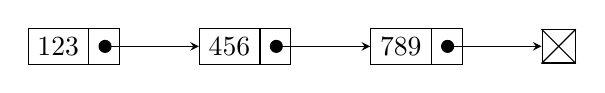
\begin{tikzpicture}[list/.style={rectangle split, rectangle split parts=2,
    draw, rectangle split horizontal}, >=stealth, start chain]

  \node[list,on chain] (A) {123};
  \node[list,on chain] (B) {456};
  \node[list,on chain] (C) {789};
  \node[on chain,draw,inner sep=6pt] (D) {};
  \draw (D.north east) -- (D.south west);
  \draw (D.north west) -- (D.south east);
  \draw[*->] let \p1 = (A.two), \p2 = (A.center) in (\x1,\y2) -- (B);
  \draw[*->] let \p1 = (B.two), \p2 = (B.center) in (\x1,\y2) -- (C);
  \draw[*->] let \p1 = (C.two), \p2 = (C.center) in (\x1,\y2) -- (D);
\end{tikzpicture}
\caption{Linked List Pre-Deletion}
\end{figure}

Suppose we want to delete $456$ from our Linked List.
\begin{itemize}
    \item Before we enter the \verb!while! loop, \verb!curr! will point to the first node (i.e. the node with data $12$), and \verb!prev! will point to \verb!null! (it will not be pointing to any node). 
    \item Next, we'll enter the \verb!while! loop since \verb!curr! does not equal null. The comparison of \verb!curr!'s data field with \verb!targetElement! will show that the two quantities are not equal, and we will subsequently move to the next iteration of the \verb!while! loop.
    \item In the second iteration of the while loop, \verb!prev! will point to the first node (i.e. the node with data $123$), and \verb!curr! will point to the second node (i.e. the node with data $456$). At this point, the comparison of \verb!curr!'s data filed with \verb!targetElement! will show that the two quantities are equal, so we will enter the \verb!if! clause. In there, we'll set the \verb!next! field of the first node equal to the third node, which ultimately results in the following Linked List: 
\end{itemize}

\begin{figure}[h]
\centering
\begin{tikzpicture}[list/.style={rectangle split, rectangle split parts=2,
    draw, rectangle split horizontal}, >=stealth, start chain]

  \node[list,on chain] (A) {123};
  \node[list,on chain] (C) {789};
  \node[on chain,draw,inner sep=6pt] (D) {};
  \draw (D.north east) -- (D.south west);
  \draw (D.north west) -- (D.south east);
  \draw[*->] let \p1 = (A.two), \p2 = (A.center) in (\x1,\y2) -- (B);
  \draw[*->] let \p1 = (C.two), \p2 = (C.center) in (\x1,\y2) -- (D);
\end{tikzpicture}
\caption{Linked List Post-Deletion}
\end{figure}

Next, we can look at a \verb!getListWithDataInBetween! function, which takes in a lower and upper bound, and it returns a Linked List with only nodes whose \verb!data! fields are between these bounds:

\begin{lstlisting}
    	public MyLinkedList<T> getListWithDataInBetween(T start, T end) {
		MyLinkedList<T> newList = new MyLinkedList<T>();

		if (head != null) {
			Node curr = head, last = null;

			while (curr != null) {
				if (curr.data.compareTo(start) >= 0 && curr.data.compareTo(end) <= 0) {
					Node newNode = new Node(curr.data);
					if (newList.head == null) {
						newList.head = newNode;
					} else {
						last.next = newNode;
					}
					last = newNode;
				}
				curr = curr.next;
			}
		}

		return newList;
	}
\end{lstlisting}

Once again, this method uses the Tom and Jerry Traversal. This method is fairly similar to the \verb!delete! method. We keep on comparing nodes until we find one that lies between our two bounds. Once such a node is found, we create a new node with the data of the current node we're at, and this node is subsequently set equal to the \verb!head! field of our newly created Linked List. 

Note that there is a special case for when we're adding the first node into our Linked List (in this case, we should make the newly created node our head). 

\subsection{Doubly Linked Lists} 

\section{Wednesday, October 10, 2019}%incomplete
\section{Wednesday, October 9, 2019}

When you have a program in Java, there are four areas of memory: the \vocab{stack}, \vocab{heap}, \vocab{static section}, and \vocab{code}. The stack is where local variables and recursive function calls are stored.

\subsection{Introduction to Recursion}

\vocab{Recursion} is a strategy for solving problems in which solutions to larger problems depend on solutions to smaller instances of the same problem. More precisely, a \vocab{recursive function} is a procedure that calls itself. The ``general" pseudocode to solving recursive problems is to solve the problem directly if it is simple or trivial enough, and otherwise simplify the problem into smaller instances of the original problem, small the smaller instances using the same algorithm, and combine the solutions to form the solution to the original problem. \\

\noindent A classical example for demonstrating recursive functions is a factorial function. Recall $n! = n(n - 1)(n - 2)\cdots (1)$. By rewriting this expression as $n! = n \cdot (n - 1)!$ (note that this is an equivalent definition), we can write a program that computes factorials as follows:

\begin{lstlisting}
/* Given an integer n, return n! */
int fact(int n) {
    if (n == 0) return 1; /* Base case */
    return n * fact(n - 1); /* Recursive step */
}
\end{lstlisting}

\noindent In this program, we've used the fact that $n!$ is equal to $n \cdot (n - 1)!$. We reduce each problem (i.e. the task of computing a factorial) into a smaller-sized subproblem (computing a factorial of a smaller number) until our problem is very easy to solve (we stop recursing when $n = 0$ is true). The case(s) in which we stop recursing and solve the problem directly are called our \vocab{base cases} (for example, here we would say ``$n = 0$ is our base case). On the other hand, the case(s) in which we continue recursing is called our \vocab{recursive step}. Another way to interpret recursive functions is a function that calls another function that does the same thing as the function we're currently in is doing. \\

\noindent We can prove that recursive algorithms work correctly through \vocab{induction}; however, we will not be proving correctness in this class. \\

\noindent What makes recursion possible? Recursion is made possible with the call stack, which is one of the four areas in memory. Essentially, the state of the current procedure or method is saved when the procedure is invoked so that we can easily restore back and continue from where we left off in a function upon encountering a recursive call. \textit{Every} function call gets its own stack space. Here is a diagram that depicts the call stack for a \verb!fact(3)! call:

\begin{figure}[h]
\centering
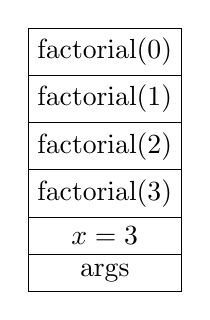
\begin{tikzpicture}[stack/.style={rectangle split, rectangle split parts=#1,draw, anchor=center}]
\node[stack=6]  {
\nodepart{one}factorial(0)
\nodepart{two}factorial(1)
\nodepart{three}factorial(2)
\nodepart{four}factorial(3)
\nodepart{five}$x = 3$
\nodepart{six}args
};
\end{tikzpicture}
\caption{Call Stack for fact$(3)$}
\end{figure}

The above diagram depicts what happens when we call the \verb!fact! function with $x = 3$. The \verb!args! and \verb!x = 3! entries are depicted in the stack just for completeness --- this is to emphasize that function calls share the stack space with local variables as well as the function ``call" to the main function. 

What are the pros and cons of using recursion? Some problems are recursive in nature, so it can be easier to implement a recursive algorithm. This means that recursive algorithms can also be simpler and easier to debug, understand, and maintain. On the other hand, having so many function calls can lead to \vocab{function overhead}, which includes the time needed to switch between functions. \\

Consider the following alternative approach to implementing the \verb!fact! method:

\begin{lstlisting}
int fact(int n) {
    int res = 1;
    for (int i = n; i > 0; i--) { res *= i; }
    return res;
}
\end{lstlisting}

This implementation of \verb!fact! is actually more efficient than the first recursive definition that we showed. The reason why we showed the first example is just for demonstration purposes.%
\section{Friday, October, 11, 2019}

\subsection{Recursive Array Functions}

In order to get a better understanding of recursion, we can show a few array-based problems in which recursion can be used as solutions. \\

\noindent Given an array and a target value, the following \verb!find()! method returns \verb!true! if the provided target value is present in the array and \verb!false! otherwise. This problem can be solved non-recursively very easily: iterate over all values, and compare each value to the provided target value. But for the sake of demonstration, we will look at the following recursive solution:

\noindent
\begin{lstlisting}
	public static boolean findElementAuxiliary(int[] array, int index, int target) {
		if (index > array.length - 1) {
			/* Empty array segment */
			return false;
		} else {
			if (array[index] == target) {
				return true;
			} else {
				return findElementAuxiliary(array, index + 1, target);
			}
		}
	}
\end{lstlisting}

In this example, we have a base case of when the Boolean expression \verb!index > array.length - 1! is true. When this logical expression evaluates to \verb!true!, our current index exceeds the size of the array. In other words, if we've gotten this far in the array without already having found the value, then we can conclude that the value does not exist in the array. On the other hand, we perform our recursive step when \verb!index <= array.length - 1! is true. In this case, we simply compare the current value at our index to the target value. If there is an equality, we return \verb!true! since we can conclude that our target value exists. If there isn't an equality, we make a recursive call to the same function with an increased index (so we will be looking at the next element in the array on the next recursive call). \\

Here's another example of a recursive function which counts the number of instances of a provided target element:

\begin{lstlisting}
	public static int instancesOfElementAuxiliary(int[] array, int index, int element) {
		if (index > array.length - 1) {
			/* Empty array segment */
			return 0;
		} else {
			if (array[index] == element) {
				return 1 + instancesOfElementAuxiliary(array, index + 1, element);
			} else {
				return instancesOfElementAuxiliary(array, index + 1, element);
			}
		}
	}
\end{lstlisting}

Once again, our base case occurs when the Boolean expression \verb!index > array.length - 1! is true. If this is true, our current index exceeds the capacity of the array, and there are no more instances of the target value. In our recursive step, we compare the current index value to the target. If there is a match, we add \verb!1! to our return value and continue looking at other elements in our array for further matches. On the other hand, if there isn't a match, we simply continue looking at other elements in our array for any further matches. \\

\noindent Intuitively, this recursive function does exactly what we would do if we were counting the number of occurrences of an element in an array by hand. We would start a counter in our head, and we would look at each index of the array in a left-to-right manner. Upon encountering a value that matches our target value, we will increment this counter and continue looking at the next elements. \\


Something that is important to note is that both of the recursive functions we've looked at so far have had an \verb!index! as a parameter. This parameter allows us to iterate through the array in a recursive fashion since we're able to keep track of where we currently are in the array. Since all initial calls to this function will have the \verb!index! parameter set equal to $0$, we can overload our recursive function as follows:

\begin{lstlisting}
public static int instancesOfElement(int[] array, int element) {
		return instancesOfElementAuxiliary(array, 0, element);
}
\end{lstlisting}

From the \verb!main!, we can now make use of the \verb!instancesOfElement! function, which only takes in an array and a target value to count. For example, we can now write \verb!System.out.println(findElement(data, 349));! instead of always having $0$ as one of the third parameters. The \verb!instancesOfElementAux! function, which performs the work to help another function, is known as an \vocab{auxillary function}.

\subsection{Recursive Linked List Functions}

In the two previous recursive array functions we've seen, we can note that we stopped iterating upon hitting the end of our array (i.e. when \verb!index > array.length - 1! is true). This is a very common base case when implementing recursive array functions since it permits us to iterate through the array until we reach the end. \\

In a similar manner, we can create recursive linked list functions whose base case occurs when we reach the end of the list. But since we don't have a \verb!.length! function anymore, we can just compare the current node that we are at to \verb!null!. \\

\noindent Here is a very simple recursive Linked List function, which simply prints a Linked List:

\begin{lstlisting}
	public void printListAux(Node headAux) {
		if (headAux != null) {
			System.out.println(headAux.data);
			printListAux(headAux.next);
		}
	}
\end{lstlisting}

We just check whether the current node we are it is \verb!null! (if this is true, then we've hit the end of the Linked List). If it is \verb!null!, we don't do anything --- no action is necessary here since we aren't returning anything. On the other hand, if the node is not null, then we print the contents of the current node, and we look at the next node with a recursive call. Consider the following Linked List:

\begin{figure}[h]
\centering
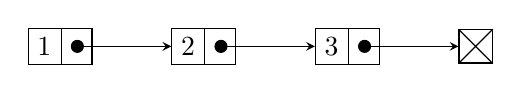
\begin{tikzpicture}[list/.style={rectangle split, rectangle split parts=2,
    draw, rectangle split horizontal}, >=stealth, start chain]

  \node[list,on chain] (A) {1};
  \node[list,on chain] (B) {2};
  \node[list,on chain] (C) {3};
  \node[on chain,draw,inner sep=6pt] (D) {};
  \draw (D.north east) -- (D.south west);
  \draw (D.north west) -- (D.south east);
  \draw[*->] let \p1 = (A.two), \p2 = (A.center) in (\x1,\y2) -- (B);
  \draw[*->] let \p1 = (B.two), \p2 = (B.center) in (\x1,\y2) -- (C);
  \draw[*->] let \p1 = (C.two), \p2 = (C.center) in (\x1,\y2) -- (D);
\end{tikzpicture}
\caption{Linked List Recursive Print Demonstration}
\end{figure}

\noindent With the use of our \verb!printListAux! function, we would end up printing \verb!1 2 3! if we passed in a representation of the above Linked List into our function. How can we modify this function to make the Linked List print in reverse order? In other words, how can we print \verb!3 2 1! instead of \verb!1 2 3!? This can be done by switching the order of the print statement and the recursive call. This way, we will recurse to the base case prior to performing any printing. \\

Now here is the Linked List analogue of the recursive \verb!find! method that we implemeneted earlier for arrays:

\begin{lstlisting}
    public boolean findAux(Node headAux, T target) {
		if (headAux != null) {
			int result = headAux.data.compareTo(target);
			return result == 0 ? true : findAux(headAux.next, target);
		}

		return false;
	}
\end{lstlisting}

This is doing the exact same thing as what our recursive array function performed. Our base case occurs once we've reached the end of the Linked List (i.e. when \verb!headAux! is \verb!null!). When we haven't hit the end of our Linked List, we check whether the current Linked List contains our \verb!target! value. If it does, we return true. Otherwise, we look at the next node. Note that in this implementation, we use the \verb!compareTo! method since our Linked List is implemented using generics. \\

Something else to keep note of is that it is important to keep our parameter name for the node (which is currently \verb!headAux!) different from the name that we have for our Linked List's \verb!head! in the Linked List class. Otherwise, the compiler will instead be referencing the \verb!head! instance variable. %
\section{Monday, October 14, 2019}

\subsection{More Recursion with Linked Lists}

Now, we can look at a more intricate example than what we have seen before. We will look at a function that takes returns an ArrayList of node entries in which the entries lie in between two provided values:

\begin{lstlisting}
    public ArrayList<T> getDataBetween(T start, T end) {
		ArrayList<T> answer = new ArrayList<T>();

		getDataBetweenAux(head, start, end, answer);

		return answer;
	}

	private void getDataBetweenAux(Node headAux, T start, T end, ArrayList<T> answer) {
		if (headAux != null) {
			if (headAux.data.compareTo(start) >= 0 && headAux.data.compareTo(end) <= 0) {
				answer.add(headAux.data);
			}
			getDataBetweenAux(headAux.next, start, end, answer);
		}
	}
\end{lstlisting}

Here, we have an auxillary function that takes in a \verb!headAux! node variable, which is used to tell us where we currently are in the array. Furthermore, we take in a \verb!start! and \verb!end! variable, and we want to add all nodes whose value lies between \verb!start! and \verb!end! into our ArrayList. \\

\noindent Similar to the previous functions we've encountered, our base case consists of checking whether we've reached the end of our Linked List. This is done by comparing \verb!headAux! to null. If we've hit the end of our Linked List, no action is necessary since our function is \verb!void! (there is nothing to return). On the other hand, if we haven't hit the end of our Linked List, we can compare the current node's data field and check whether it lies between the \verb!start! and \verb!end! values provided. If it does, we can add this value into our \verb!ArrayList!. \\

The approach taken by this recursive method differs from what we've seen before. In previous recursive functions, when we were returning an integer, boolean, or simply printing values, we would have a \verb!return! statement that would give us what we wanted from the function. In this function, however, we pass in an empty ArrayList which gets modified into what we want. This implementation allows us to not have to keep track of all of the elements that lie between the \verb!start! and \verb!end! values provided since we're adding the value immediately after this condition is satisfied (this gives our function a ``memoryless" property). \\

\subsection{Tail Recursion}

\vocab{Tail recursion} is a type of recursive function in which we do not need to perform any further actions on a recursive call. In other words, a tail recursive function is a recursive function in which the function calls itself at the end (the ``tail" of the function) of the function in which no computation is done after the recursive call. For example, the \verb!getDataBetweenAux! function that we just saw is tail recursive because no further processing is necessary once we've made the last recursive call. On the other hand, the \verb!instancesOfElementAuxillary! function that we saw for arrays is not tail recursive since we might need to add $1$ to the value returned by the recursive call. \\ 

\noindent Why do we care about tail recursion? Mostly because using tail recursion allows us to write more optimized code.  Since tail recursive functions don't have any processing after their recursive calls, there is no need to actually store the current function in the stack. Instead, we can save some memory and only store the recursive call. \\


\subsection{Common Recursion Problems}

Some common recursion-related problems that one may encounter are listed below:

\begin{itemize}
    \item Infinite recursion: This problem can occur if our recursive step does not simplify the original problem into a smaller-sized subproblem. We can also encounter infinite recursion when we forget to include a base case. For example, something like, \verb!int bad(int n) { if (n == 0) return bad(n-1); }! is an example of infinite recursion since we will keep calling this function without terminating. Eventually, our program halts when our stack runs out of memory from our recursive calls. This is known as a \vocab{stack overflow}. 
    \item Efficiency: Just because recursion works doesn't mean it's the best solution. This is particularly true since recursive functions often perform the same work over and over again. 
\end{itemize}

\subsection{Introduction to Hashing}

\vocab{Hashing} is a technique used for storing key-value entries into the array. The process of hashing is utilized by \vocab{hash tables}, which are data structures that allow us to ideally insert and retrieve values in constant time.  For example, let's say there's a collection of objects and a data structure needs to answer queries of the form ``Is this object in the data structure?" (e.g. is this word in the dictionary?).  By using hashing, we can do this in less time than it takes to perform a binary search. \\

How is hashing performed? The idea is to first find a function (known as a \vocab{hash function}) that maps the elements of the provided collection to an integer between $1$ and $N$, where $N$ is some number larger than the number of elements in your collection. For example, if you want to store the characters \verb!'a'!, \verb!'b'!, and \verb!'c'!, then we require $N \geq 3$. Now, we can keep an array indexed from $1$ to $N$ (so we have an array of size $N$), and we can store each element at the position that the function evaluates the element as. So if our hash function is $f(x)$ and $f(a) = 1$, $f(b) = 2$, and $f(c) = 3$, then we would store \verb!'a'! in index $1$, and so on. Now, what if we want to determine if an element is present in our data structure? This is also simple: just plug in the value we want to check into our function, and check whether the element is present in the index computed. \\

What are some desirable properties of hash functions?
\begin{itemize}
    \item A hash function should be quick to compute. This is true because we want our hash table data structure to support quick retrieval and storing of data. If it takes too much time to compute the index of where a value of interest resides, our hash table itself will run slowly when computing indices of where data should reside.
    \item A hash function should \vocab{collision-free}. This means that it should be difficult to produce two distinct keys that map to the same value. On the extreme end, suppose we had a function that \textit{always} produced $1$, no matter what value was provided to it. This means that multiple values would get mapped to the first index in the array, which is not desirable. A function that produces \textit{no collisions} is called a \vocab{perfect hash function}.  
    %A hash function being collision-free is a desirable property because, otherwise, multiple keys would map to the same index in the array.  On the extreme end, we say a hash function is \vocab{ideal} if every search key corresponds to a unique element in the hash table. Using a function that distributes values approximately uniformly reduces the probability of collisions occurring.
\end{itemize}


So, what are some examples of good hash functions? Typically, it's a good idea to create a relatively huge value and use the modulus operator in order to reduce it to the size of our array (the process of reducing this value to the size of the array is referred to as \vocab{scaling}). This works particularly well when our hash table's size is a prime number. \\

In Java, we can generate a \vocab{hash code} (the value produced by the hash function, prior to reducing it to the size of the array with the modulus operator) for a string by using the built-in \verb!.hashCode()! function:

\begin{lstlisting}
System.out.println("Java".hashCode()); // Prints 2301506.
\end{lstlisting}

How does \verb!"Java"! produce $2301506$?. The ASCII value for J, a, and v are $74, 97$, and $118$, respectively. The hashCode is then computed by $74 \cdot (31)^{3} + 97 \cdot (31)^{2} + 118 \cdot 31 + 97 = 2301506$. \\

This is an example of how hash codes can be computed on strings. For primitive types, like floats or doubles, hash functions typically manipulate the internal binary representation to produce a hash code. For practical purposes, it's usually not plausible to produce a perfect hash function that produces distinct values for every key. In pratice, it's good to pick something that seems fairly random and verify that it works.


\section{Wednesday, October 16, 2019}

Last time, we introduced hash tables in which certain keys are mapped to indices where their corresponding values reside with the use of a function. What happens if our hash table runs out of space? In order to resolve this issue, we can create a new hash table with greater size and rehash all of our values. 

\subsection{Resolving Collisions}

As we have mentioned, it is desirable to have a hash function that prevents collisions. But what happens if a collision \textit{does} occur? We can't store two values in the same index in the array, and our data structure would be unreliable if we just replaced the old value (or didn't store the new value). There are two primary ways in which we can resolve collisions known as \vocab{open addressing} and \vocab{separate chaining}. In open addressing, we look for an unused entry in the table. In separate chaining, each element in the table becomes associated with more than one search key (i.e. each element becomes a bucket or a list). \\

\subsubsection{Open Addressing}
Open addressing can further be subdivided into several variations. A common theme between these variations is that they all use \vocab{probing}, which is the process for locating an open element or position in the hash table. Suppose our hash table has size $n$. \\

\noindent One type of open addressing is known as \vocab{linear probing}. In this variation, when a collision occurs at some index position $k$, we look to see whether position $k + 1 \pmod{n}$ is available (not in use) If it is in use, we look at $k + 2 \pmod{n}$, and so on. Suppose we want to keep a hash table of strings, and our hash function evaluates the following:
\begin{itemize}
    \item \verb!hash("apple") = 5!
    \item \verb!hash("watermelon") = 3!
    \item \verb!hash("kiwi") = 0!
    \item \verb!hash("mango") = 6!
    \item \verb!hash("banana") = 2!
    \item \verb!hash("orange") = 3!
    \item \verb!hash("pear") = 3!
\end{itemize}

Under linear probing, we would end up with the following hash table:

\begin{figure}[h]
\centering
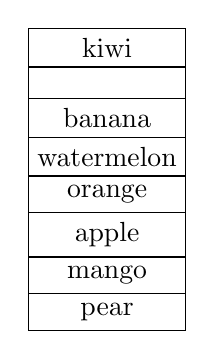
\begin{tikzpicture}[stack/.style={rectangle split, rectangle split parts=#1,draw, anchor=center}]
\node[stack=8]  {
\nodepart{one}kiwi
\nodepart{two}
\nodepart{three}banana
\nodepart{four}watermelon
\nodepart{five}orange
\nodepart{six}apple
\nodepart{seven}mango
\nodepart{eight}pear
};
\end{tikzpicture}
\caption{Linear Probing Example}
\end{figure}

How do we get this hash table? 
\begin{itemize}
    \item First, we insert \verb!apple! into index $5$ (our indices start from $0$, where index $0$ is the top-most entry), \verb!watermelon! into index $3$, \verb!kiwi! into index $0$, \verb!mango! into index $6$, and \verb!banana! into index $2$. 
    \item Next, we encounter a collision between \verb!orange! and \verb!watermelon!. But using linear probing, we can resolve this collision by noting that index $4$ is empty. Thus, \verb!orange! is moved into index $4$.
    \item Next, we encounter a collision between \verb!watermelon! and \verb!pear!. We find the next available index, which is index $7$, so we place \verb!pear! into index $7$. 
\end{itemize}

As you may have noticed, resolving collisions with linear probing generates groups of consecutive elements in the hash table. Each group is called a \vocab{cluster}, and this phenomenon is known as \vocab{primary clustering}. Bigger clusters means longer search times since for each cluster is a sequence of probes that we must search when adding, removing, or retrieving.


Another type of open addressing is known as \vocab{quadratic probing}. In this case, we consider elements at indices $k + j^{2} \pmod{n}$. For example, we'd first look at index $k + 1 \pmod{n}$ followed by $k + 4 \pmod{n}$, $k + 9 \pmod{n}$, and so on. Unlike linear probing, quadratic probing does not result in primary clustering. Instead, it results in \vocab{secondary clustering}, which is a phenomenon in which filled slots are mapped to values that are far away from their keys. \\

\noindent Finally, one last variant is \vocab{double hashing} in which the increment of $1$ for linear probing and $j^{2}$ for quadratic probing is replaced with the result of a second, different hash function that determines the increment. \\

\subsubsection{Separate Chaining}

Separate chaining is a second approach to resolving collisions. In this case, each element of the table represents more than one value. Each element in the hash table is called a \vocab{bucket}, which can be represented internally with a list, sorted list, or a linked list, etc. Buckets should support searching: we should be able to determine the bucket by hashing the search key and look through the list to find the element or determine that it does not exist. Also, buckets should support insertion: we should look for an item and insert it into the found bucket if it is not found. Finally, buckets should support removal: we should be able to look for the item and remove it from the bucket. \\

It is important that the number of elements in each bucket is very small. Equivalently, it is important that we do not have too many collisions. Otherwise, we might end up having to search a large list, which completely defeats the purpose of using a hash table. For example, consider the extreme case in which \textit{every} value resides in index $1$. In this case, we'll need to search a list in the worst case, which makes a hash table no better than just using an array or a Linked List. 

\subsection{Load Factor}

We can quantify the cost of collision resolution with a statistic known as the \vocab{load factor}. The load factor is denoted by $\lambda$ and it is defined as follows:

\begin{align*}
\lambda = \frac{\text{number of entries in hash table}}{\text{size of the hash table}}.
\end{align*}

As $\lambda$ increases, the number of comparisons needed to resolve collisions also increases. The performance of linear probing degrades the load factor increases. In order to keep reasonable efficiency, we should maintain $\lambda \leq 0.5$ (i.e. the hash table should be less than half full).  \\

Once we have $\lambda > 0.5$, it is typically useful to resize the hash table and compute a new hash index for every key. This process is known as \vocab{rehashing}.

\subsection{Hash Code Contract}

In Java, when we're using hash functions, we must satisfy something known as the \vocab{hash code contract}. Essentially, this contract states that if \verb!a.equals(b)! evaluates to true, then we must guarantee \verb!a.hashCode() = b.hashCode()!. However, the inverse or converse of this statement do not necessarily have to be true. That is, it is not necessary for \verb@!a.equals(b)@ to imply \verb@a.hashCode() != b.hashCode()@, and it is not necessary for \verb@a.hashCode() == b.hashCode()@ to imply \verb@a.equals(b) == true@. \\

Note that these conditions imply that hash functions must be deterministic in the sense that we should always get the same hash whenever we compute the hash code of an object. 

\subsection{HashSets}

Java provides us with a a \verb!HashSet! as a part of the \verb!Collections! framework. The \verb!HashSet! creates a collection that internally uses a hash table for storage. Here is an example of how we can use a \verb!HashSet!:

\begin{lstlisting}
package setIncorrect;

import java.util.*;

public class Roster {
	private HashSet<Person> roster = new HashSet<Person>();

	public void addPerson(String name, int id) {
		roster.add(new Person(name, id));
	}

	public boolean findPerson(String name, int id) {
		Person person = new Person(name, id);
		
		return roster.contains(person);
	}
}
\end{lstlisting}

Here, we are using a \verb!HashSet! to represent a collection of \verb!Person! objects. The \verb!addPerson! function adds another \verb!Person! object into our \verb!HashSet! with the provided name and ID. Internally, this \verb!Person! object is added into our hash table. The \verb!findPerson! method performs an internal look-up in our hash table, and checks whether a \verb!Person! object with the same name and ID already exists. \\

Now consider the following driver program:

\begin{lstlisting}
package setIncorrect;

public class Driver {
	public static void main(String[] args) {
		Roster section0101 = new Roster();

		section0101.addPerson("Mary", 10);
		section0101.addPerson("Peter", 20);
		section0101.addPerson("Jose", 7);

		if (section0101.findPerson("Peter", 20)) {
			System.out.println("Found Peter");
		} else {
			System.out.println("Peter not found");
		}
	}
}
\end{lstlisting}

In this driver, we add three different \verb!Person! objects into the \verb!HashSet! corresponding to our \verb!Roster!. In other words, we compute a hash code for each of our objects, and we store them into a large array. By default, the hash code corresponding to a user-made object is just the object's memory address --- we can easily verify that this satisfies the hash code contract since \verb!a.equals(b)! implies \verb!a! and \verb!b! reside in the same memory location. \\ 

Next, in our code, we check whether our \verb!HashSet! contains a \verb!Person! object with name \verb!"Peter"! and Id \verb!20!. In other words, we compute the hash code for this object, and we check whether there is an entry in our hash table at this index. Assuming our hash function satisfies the hash code contract, this expression evaluates to true, so we print \verb!"Found Peter"!.  \\

It is important to emphasize that, ideally, this is more efficient than using a simple array-based implementation. We are able to retrieve and store elements in expected constant time, which is better than having to iterate through the entire array to find a \verb!Person! object. 


\section{Friday, October 18, 2019}

Exam $2$ today.
\section{Monday, October 21, 2019}


\subsection{Recap on Java's Hash Code Contract} 

In order to recap what we learned last week, we can review Java's Hash Contract. \\

\noindent Java's Hash Code Contract states that if two objects are equal (using the \verb!.equals()! method), then we must guarantee that their hash codes are also equal. What happens if we don't satisfy the hash code contract? Classes that rely on hashing will fail. 

When we write our own classes, we must write classes that satisfy Java's Hash Code Contract. We will run into problems if we don't satisfy the Java Hash Code Contract and use classes that rely on hashing (like \verb!HashSet! or \verb!HashMap!). A possible problem that we might run into is being able to add elements to a set but not being able to find it during a lookup operation.  \\

It is also useful to be able to recognize when valid hash functions are bad. For instance, overriding the \verb!hashCode()! method to make it \textbf{always} return $5$ is a a valid hash code. Why? Because if \verb!a.equals(b)! is true, then \verb!a.hashCode() = b.hashCode()! is also true (\verb!a.hashCode()! and \verb!b.hashCode()! will always evaluate to $-5$). But this hash code is not good because we will have many collisions -- many elements are being mapped to index $5$. 

\subsection{Sets and Maps}

A \vocab{set} is a collection that cannot contain duplicate elements. Two set instances are considered to be equal if they contain the same elements. Java's Collections library contains three general-purpose set implementations:
\begin{itemize}
    \item The \verb!HashSet! set is implemented with hashing. We have already seen this in use in our \verb!Roster! example. The elements in the \verb!HashSet! must implement the \verb!hashCode()! method. This type of set provides us with the most efficiency (in terms of time). 
    \item The \verb!LinkedHashSet! is a \verb!HashSet! that supports the ordering of elements. This allows us to retrieve elements in the order in which we inserted them. On the other hand, the \verb!HashSet! does not guarantee any type of ordering. 
    \item The \verb!TreeSet! guarantees that the elements in a set are in sorted order. The elements being stored in a \verb!TreeSet! must be comparable. We can also pass in custom comparators when using a \verb!TreeSet!. 
\end{itemize}

A \vocab{map} is an abstract data type that holds (key, value) pairs. We can think of maps as arrays except we aren't constrained to using integers as our indices. Instead, we can use any other type to index other values, like strings to other strings. The map interface provides methods like \verb!put(K key, V value)! to insert an element, and \verb!get(Object key)! to retrieve an element. There is also a \verb!remove(Object key)! and \verb!clear()! function to remove a single element or completely clear the map. The map concrete classes are listed below. Note that the \verb!Map! interface is not a subtype of the \verb!Collection! interface:

\begin{itemize}
\item The \verb!HashMap! map is implemented using hashing. Elements must satisfy the \verb!hashCode()! contract. The \verb!HashMap! is the most efficient in terms of time.
\item The \verb!LinkedHashMap! supports ordering of elements (we can retrieve elements in order of insertion), but it is slower than the \verb!HashMap!, which does not guarantee any type of ordering. 
\item The \verb!TreeMap! requires elements to be comparable, and it guarantees that elements can be retrieved in sorted order.
\end{itemize}

The following example demonstrates the differences between the three types of maps, and it also illustrates some of the primary methods that we use with maps:

\begin{lstlisting}
/*
 * Example that shows how we can use maps.
 */
import java.util.*;
public class ClassesImpMaps {
	
	public static void main(String[] args) {
		System.out.println("************* HashMap test *************");
		test(new HashMap<>());
	
		System.out.println("\n\n************* TreeMap test *************");
		test(new TreeMap<>());
		
		System.out.println("\n\n************* LinkedHashMap test *************");
		test(new LinkedHashMap<>());
	}
	
	/* Notice the parameter is a Map, which is an interface */
	public static void test(Map<String, Department> map) {
		
		/* adding <key,value> pairs to the map */
		map.put("Mary", new Department("Electronics", 5000));
		map.put("Peter", new Department("Music", 4500));
		Department shoeDepartment = new Department("Shoe", 6000);
		map.put("Zoe", shoeDepartment);
		map.put("Laura", shoeDepartment);
	
		/* printing the contents */
		Set<String> nameSet = map.keySet();
		for (String name : nameSet) { 
			/* finding the dept that maps to the name */
			Department dept = map.get(name);
			System.out.println(name + " " + dept); 
		}
		
		/* Membership test */
		if (map.containsKey("Mary"))
			System.out.println("Mary found");
		
		if (!map.containsKey("Laura"))
			System.out.println("Laura not found");
		
		/* Getting all the values */
		System.out.println("All departments");
		Collection<Department> collection = map.values();
		for (Department dept : collection) {
			System.out.println(dept);
		} 
		
		/* Another alternative */
		System.out.println("*Another alternative*");
		for (Map.Entry<String, Department> elem : map.entrySet()) {
			System.out.println(elem.getKey() + " " + elem.getValue());
		}
	}
}
\end{lstlisting}

In the \verb!test! function, we take in a \verb!Map! that maps \verb!String! objects to \verb!Department! objects. Since we only specify that the parameter is a \verb!Map!, it is valid for us to pass in a \verb!HashMap!, \verb!TreeMap!, or even a \verb!LinkedHashMap!. In this example, we are mapping employee names to departments in which they work in. The \verb!test! function adds four entries to this map. Firstly, we add \verb!Mary! and \verb!Peter! who work in the \verb!Electronics! and \verb!Music! departments, respectively. Next, we add \verb!Zoe! and \verb!Laura! both of whom work in the \verb!shoeDepartment!. \\

Next, we store the map's \verb!.keySet()! in the variable \verb!nameSet!, which is a function returns a \verb!Set! of keys stored in the map. By using an enhanced for-loop, we can iterate over \verb!nameSet!, but we are not guaranteed any type of ordering. \\

In our ``membership test" section, we will find that the Boolean expression \verb!map.containsKey("Mary")! evaluates to true, whereas the Boolean expression \verb!map.containsKey("Laura")! evaluates to false. Finally, we provide two different ways in which we can print the values in the map. 

%
\section{Wednesday, October 23, 2019}

Last time, we started looking at the classes that implement the maps, and we looked at a word frequency counter that counts the number of times a word appears in an array of strings.

\subsection{Applications of Maps and Sets}

The following example demonstrates a basic application of maps in which we count the number of occurrences of words in an array of strings:

\begin{lstlisting}
public class WordFrequencyCounter {
	public static void main(String[] args) {
		Map<String, Integer> map = new TreeMap<>();
		
		for (String word : args) {
			if (!map.containsKey(word)) {
				map.put(word, 1); /* First instance seen */
			} else {
				map.put(word, map.get(word) + 1);
			}
		}
		
		System.out.println("Words Frequency:\n");
		for (String word : map.keySet()) {
			System.out.println(word + "\t" + map.get(word));
		}
	}
}
\end{lstlisting}

Here, we create a \verb!Map! that maps \verb!String! objects to \verb!Integer! objects. More precisely, we will be mapping words to the number of times they appear in an array. Next, we process every element in the array \verb!args! with an enhanced for-loop. For every word in the provided string array, we check whether we've seen the word before. If so, we increment the integer that it is being mapped to by one. Otherwise, we set its entry to $1$ since it has only occurred once at the given time. Note that it is important that we handle these two cases separately since it would be an error to increment the value if it has not yet been declared (the default value is not $0$!).  

Finally, we print out the frequency of all of the words. Since we are using a \verb!TreeMap!, we are guaranteed that we will print the words in a sorted manner. 

% end of ex

Next, here's an implementation of a \verb!Course! object in which we use a maps and sets:

\begin{lstlisting}
package maps;

import java.util.*;

public class Course {
	private Map<Integer, Set<String>> allSectionsMap = new HashMap<>();

	public void addStudent(Integer sectionNumber, String name) {
		Set<String> sectionSet = allSectionsMap.get(sectionNumber);

		if (sectionSet == null) {
			sectionSet = new TreeSet<>();
			allSectionsMap.put(sectionNumber, sectionSet);
		}
		sectionSet.add(name);
	}

	public boolean removeStudent(String name) {
		for (Integer sectionNum : allSectionsMap.keySet()) {
			Set<String> sectionSet = allSectionsMap.get(sectionNum);
			
			if (sectionSet.contains(name)) {
				sectionSet.remove(name);
				if (sectionSet.isEmpty()) {
					allSectionsMap.remove(sectionNum);
				}
				return true;
			}
		}

		return false;
	}

	public void printAllStudents() {
		for (Integer sectionNum : allSectionsMap.keySet()) {
			Set<String> sectionSet = allSectionsMap.get(sectionNum);
			
			for (String name : sectionSet) {
				System.out.println(name);
			}
		}
	}

	public static void main(String[] args) {
		Course course = new Course();

		course.addStudent(201, "Jose");
		course.addStudent(101, "Mary");
		course.addStudent(101, "Kelly");
		course.printAllStudents();
	}
}
\end{lstlisting}

In this implementation, we use a \verb!Map! to map integers to a \verb!Set! of strings. In the context of this class, we are mapping section numbers (which fully determine a course) to a \verb!Set! of student names, representing the people taking that course. \\

In the \verb!addStudent! method, we take in a section number as well as the student to add. We retrieve the current set of students by using our \verb!Map!'s \verb!.get()! method. Subsequently, we check to see if the retrieved value is \verb!null!. This is important because, as mentioned in the previous example, there is no default value for what the keys are being mapped to. This means that we can obtain a \verb!NullPointerException! if we don't handle the case in which the \verb!sectionNumber! has no students separately. \\

If the \verb!sectionSet! retrieved is null, then the class is currently empty. This means that we need to instantiate a set, make the \verb!sectionNumber! map to the \verb!sectionSet!, and finally add the student's name to the \verb!setctionSet!. On the other hand, if the \verb!sectionSet! is not null, then we can just add the student without any trouble. \\

In the \verb!removeStudent! method, we iterate over all of the section numbers (i.e. all of the keys) by using the \verb!keySet! method of our map. For every key we iterate over, we retrieve the set corresponding to that key, and we check whether that student is in that course. If so, we remove the student from that course. If the course becomes empty after removing that student (that is, the student was the only student in that course), then we remove the course as well. \\

Finally, the \verb!printAllStudents()! function iterates over all section numbers. For each section number, retrieve the set of students in that course. Finally, we print the names of the students in each course.  \\


Another example in which maps can be useful is by using lists as keys. Consider the following code segment: 


\begin{lstlisting}
package maps;

import java.util.HashMap;
import java.util.List;
import java.util.ArrayList;

public class ListsAsKeys {
	public static void main(String[] args) {
		HashMap<List<String>, String> favoriteDessertMap = new HashMap<>();

		ArrayList<String> johnSmith = new ArrayList<>();
		johnSmith.add("John");
		johnSmith.add("Smith");
		favoriteDessertMap.put(johnSmith, "Chocolate");

		ArrayList<String> rosePeterson = new ArrayList<>();
		rosePeterson.add("Rose");
		rosePeterson.add("Peterson");
		favoriteDessertMap.put(rosePeterson, "Ice Cream");

		for (List<String> list : favoriteDessertMap.keySet()) {
			System.out.println(list + " " + favoriteDessertMap.get(list));
		}

		/* Retrieving */
		ArrayList<String> temp = new ArrayList<>();
		temp.add("John");
		temp.add("Smith");
		if (favoriteDessertMap.containsKey(temp)) {
			System.out.println("Favorite Dessert John Smith: " + favoriteDessertMap.get(temp));
		}

		/* Notice what happens when we cleared the entry */
		johnSmith.clear();
		System.out.println("Listing Map Contents After Clearing: ");
		for (List<String> list : favoriteDessertMap.keySet()) {
			System.out.println(list + " " + favoriteDessertMap.get(list));
		}
	}
}
\end{lstlisting}

In this example, we created a \verb!HashMap! that is mapping a list of people's names (represented as \verb!String! objects) to another \verb!String! object representing their favorite food. There aren't too many new concepts going on, except that it might seem counterintuitive to use a \verb!List! as our key. Near the bottom of the code segment, after we've cleared \verb!johnSmith()!, we print out \verb![], null!. The \verb![]! indicates an empty array, and the \verb!null! indicates that the corresponding value is not present. This emphasizes that it is important not to mess with the keys that are being used. 
\section{Friday, October 25, 2019}

\subsection{Algorithmic Complexity}

\subsubsection{Time Functions and Big-$\O$ Notation}
While we have already looked at the basics of Big-$\mathcal{O}$ notation, we will now learn how to analyze programs and determine their asymptotic complexity on our own. 

The \vocab{critical section} of a program is another word for the ``heart" of an algorithm. In essence, it indicates the portion of code where the most ``work" is performed in terms of time needed. The critical section of an algorithm dominates its overall execution time, and its operation is central to the functioning of a program. Typically, the sources of a critical section comes from loops or recursion.

Our goal is to find the asymptotic complexity of various algorithms. The general approach for doing so is ignoring frequently executed parts of the algorithm, finding the critical of the algorithm, and determining how many times the critical section is executed as a function of the problem size. 


Here's an example of some code in which we can easily identify the critical section:

\begin{lstlisting}
A
for (int i = 0; i < n; i++) {
    B /* This is the critical section. */
}
C
\end{lstlisting}

Suppose $A$, $B$, and $C$ are sequences of constant-time operations (for example, print statements). Then, $A$ is executed exactly once, $B$ is executed $n$ times (it is inside of a loop that loops through $n$ times), and $C$ is executed exactly once. Therefore, the total number of operations we perform is $T(n) = 1 + n + 1 = n + 2$. The high-order term of $T(n)$ is $n$, which implies that this algorithm runs in $\O(n)$ time. The function $T(n)$, which gives the exact number of operations, is referred to as our \vocab{time function}. Using this terminology, our asymptotic complexity is the high-order term of our time function. \\

It is important to be able to compute the time function exactly. Thus, it is important to be careful, particularly with the bounds of our loops. In the previous example, it is clear that the loop iterates through exactly $n$ times (once for $i = 0$, once for $i = 1$, all the way up to $i = n - 1$). If we instead wrote our loop as \verb!for (int i = 1; i <= n; i++)!, then our loop would still iterate through $n$ times. But \verb!for (int i = 0; i <= n; i++)! iterates through $n + 1$ times. Another example of a for-loop is given by \verb!for (int i = 0; i < n; i += n)!, which executes only once. \\


Here's another example:

\begin{lstlisting}
A
for (int i = 0; i < n; i++) {
    B
    for (int j = 0; j < n; j++) {
        C
    }
}
D
\end{lstlisting}

Once again, suppose $A, B, C, D$ are sequences of constant-time operations. In this scenario, $A$ is executed exactly once. $B$ is executed exactly $n$ times (it is in a for-loop that iterates through $n$ times), $C$ is executed $n^{2}$ times (it is inside a for-loop that executes another for-loop that iterates $n$ times exactly $n$ times, so we have $n \cdot n = n^{2}$ executions).  Finally, $D$ is executed once. Therefore, our time function is given by
\[
T(n) = 1 + n + n^{2} + 1 = n^{2} + n + 2.
\]

The high-order term of $T(n)$ is $n^{2}$, so this algorithm runs in $\O(n^2)$ time.  \\

Here is a third example:

\begin{lstlisting}
A
for (int i = 0; i < n; i++) {
    for (int j = i + 1; j < n; j++) {
        B /* Critical section. */
    }
}
\end{lstlisting}

Here, $A$ is executed exactly once. But now, the inner for-loop depends on the value of the outer for-loop. How do we determine the number of times $B$ is executed? We can note that when $i = 0$, the inner for-loop starts at $j = 1$, and it goes up to $n$. This contributes a total of $(n - 1)$ executions. Next, when $i = 1$, the inner for-loop starts at $j = 2$, and goes up to $n$. This contributes a total of $(n - 2)$ executions. This process continues up until the inner for-loop contributes $0$ executions. Therefore, our time function is given by
\begin{align*}
T(n) &= \underbrace{1}_{\text{Executions of Statement $A$}} + \underbrace{\left((n - 1) + (n - 2) + \cdots + 1 + 0\right)}_{\text{Executions of Statement $B$}} \\[1em]
&= 1 + \frac{n(n - 1)}{2} \\[1em]
&= \frac{n^2}{2} - \frac{n}{2} + 1
\end{align*}

\noindent where we used the identity $\sum_{k=1}^{n} k = n(n + 1)/2$ to simplify the number of executions of Statement $B$. Since the high-order term of of $T(n)$ is $n^2$, we conclude our algorithm is $\O(n^{2})$. 

\noindent It is important to note that minor changes to algorithms won't affect the asymptotic complexity of the algorithm. For example, if we instead looped from $i = 0$ and $j = i + 1$ up to $n/2$ instead of $n$, our algorithms would still be $\O(n^2)$ (although, our time functions would decrease). Essentially, Big-$\O$ notation is mostly concerned with \textit{long-run} behavior, whereas time functions are concerned with exact behavior. \\

Here is another example:

\begin{lstlisting}
int i = 1;
while (i < n) {
    /* This is the critical section. */
    A
    i = 2 * i;
}
B;
\end{lstlisting}

\noindent In this case, the statement $i = 1$ contributes $1$ to our time function (the time function accounts for \textit{every} operation). Now, how many times does $A$ execute? The answer is $\log_{2}(n)$. This can be seen easily by plugging in different powers of $2$ for $n$, and tracing the code. Logarithmic time complexity typically indicates that we are increasing the loop variable by some constant factor, or we're reducing the problem at-hand by a constant factor. Thus, statement $A$ contributes a $\log_2(n)$ term to our time function, and the re-assignment of $i$ inside of the for-loop contributes another $\log_2(n)$ term. Finally, the statement $B$ executes one more operation, from which we obtain
\[
T(n) = 1 + \log_2(n) + \log_2(n) + 1 = 2(\log_2(n) + 1).
\]

\noindent The high-order term here is $\log(n)$ so we conclude that this algorithm is $\O(\log(n))$. \\

\subsection{Complexity of Recursive Algorithms}

How can we compute the complexity of a recursive algorithm? We can do this by writing the recurrence in terms of itself. For example, consider the following program:

\begin{lstlisting}
int fact(n) {
    if (n == 0) return 1;
    return n * fact(n - 1);
}
\end{lstlisting}

If $n$ is greater than $0$, then we perform exactly $3$ operations and perform a recursive call on $n - 1$. On the other hand, if $n$ is equal to $0$, then we perform only one operation. In this case, our time function can be expressed by $T(n) = T(n - 1) + 3$ with base case $T(1) = 0$. This type of equation is known as a \vocab{recurrence}. There are many ways to solve recurrences, but knowing how to solve them is not necessary in this class. \\

\noindent By performing iteration, we can solve the recurrence in a very informal way by identifying a pattern:

\begin{align}
T(n) &= T(n - 1) + 3 \\
&= T(n - 2) + 6 \\
&= T(n - 3) + 9 \\
&= \ldots \\
&= T(n - k) + 3k.
\end{align}

We keep on iterating until $k = n$ in which case we obtain $T(n) = T(0) + 3n$. But since we have the base case $T(0) = 1$, we find $T(n) = 3n + 1$. Therefore, we can conclude that the algorithm runs in$\O(n)$ time. \\


Here's another example of an algorithm (pseudocode is shown):

\begin{lstlisting}
MergeSort(Array) {
    if (n == 1) return;
    MergeSort(first half of array)
    MergeSort(second half of array)
    Merge the two halves. /* Requires n operations. */
}
\end{lstlisting}

In this algorithm, we perform $n$ operations per recursive call. In addition, we make two calls to the algorithm with subproblem size $n/2$, so we obtain $T(n) = 2T(n/2) + n$ as our recurrence equation. The base case occurs when $n = 1$ in which case we perform just one operation. Thus, our base case is given by $T(1) = 1$.  This recurrence can be a little bit more tricky to solve, but the solution's high order term is $n\log_{2}(n)$. Thus, this algorithm runs in $\O(n\log(n))$ time. 


\subsection{Additional Complexity Measures}

So far, we have only discussed Big-$\O$ notation, which is an upper bound on the number of operations we perform. However, we can also use Big-$\Omega$ notation, which is a \textit{lower} bound on the number of operations we perform (e.g. what is the least number of operations we perform?). \\

\noindent Suppose we want to find the maximum element in an array with $n$ numbers. One easy way to do this is to keep track of the maximum value seen so far, and update this value when we see a new maximum. This algorithm runs in $\O(n)$ time. But, it can also be shown that a lower bound for this algorithm is $\Omega(n)$ time. This is true because there cannot exist an algorithm that finds the maximum of $n$ numbers without at least looking at what the $n$ numbers are. But even the act of just looking at the $n$ numbers requires linear time. \\

When the Big$-\O$ and Big-$\Omega$ of an algorithm are equal (i.e. $\Omega(f(n)) = \O(f(n))$ for some function $f(n)$), then we say that the algorithm is $\Theta(f(n))$. This is a stronger result. 


\subsection{Trees}
A \vocab{tree} is a hierarchical, non-linear data structure that can be used to represent a one-to-many relationship between elements. The data structure consists of a \vocab{root node} which is typically the topmost node in a data structure as well as many other \vocab{internal nodes}. Each node stores values and references to other nodes in the tree. Below is an example of a tree:

\begin{figure}[h]
\centering
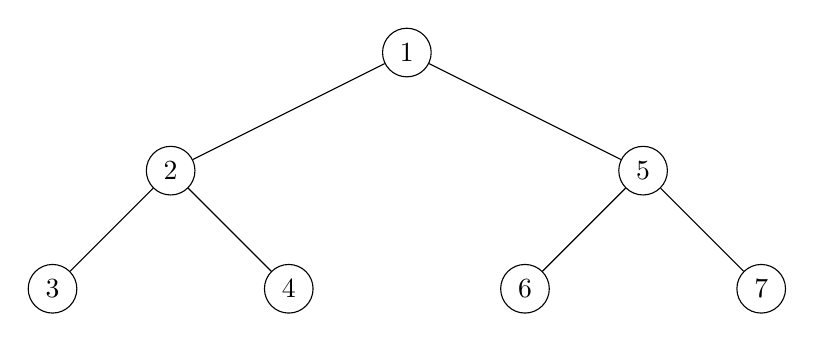
\begin{tikzpicture}[level/.style={sibling distance=60mm/#1}]
\node [circle,draw] (z){$1$}
  child {node [circle,draw] (a) {$2$}
    child {node [circle,draw] (b) {$3$}
    }
    child {node [circle,draw] (g) {$4$}}
  }
  child {node [circle,draw] (j) {$5$}
    child {node [circle,draw] (k) {$6$}
    }
  child {node [circle,draw] (l) {$7$}}
};
\end{tikzpicture}
\caption{An Example of a Tree}
\end{figure}

Here, the node labelled $1$ is the root node, and every other node is an internal node. 

What are trees useful for? Trees are good for clearly depicting relationships. For example, we can model ancestry trees, or relationships between people. We can also model a network of cities with vertices representing cities, and an edge between two cities representing a roadway or path between the two cities.

In the diagram above, we see that every node other than $3, 4, 6$ and $7$ have two nodes coming out, underneath them. We call these nodes the \vocab{child nodes} of the node that they are coming out of (so nodes $3$ and $4$ are the children of node $2$, and node $7$ has no children). Also, we can differentiate between the two children by using the terminology \vocab{left child} and \vocab{right child}. 

The \vocab{level} of a node is a measure of the node's distance from the root. More precisely, if the node is the root of the tree, then its level is $1$. Otherwise, its level is its parent's level plus one. The \vocab{height} of a tree is the maximum level of any node in the tree. \\

A \vocab{binary tree} is a special kind of tree in which each node has at most $2$ children. We will place a special focus on this type of tree, starting next lecture. 
\section{Monday, October 28, 2019}
asdf

\section{Number Theory}
Prime Sieve
\begin{lstlisting}
#include<iostream>
#include<bitset>

int main(int argc, char** argv) {
 std::bitset<1000> sieve;
 for(int i = 2; i < sieve.size(); i++) {
  if(!sieve[i]) {
   for(int j = i * i; j < sieve.size(); j += i) {
    sieve[j] = true;
   }
  }
 }

 // Printing all primes
 for(int i = 2; i < sieve.size(); i++) {
  if(!sieve[i])
   std::cout << i << "\t";
  if(!(i % 40))
   std::cout << std::endl;
 }
 std::cout << std::endl;
}
\end{lstlisting} 

ModPow

\begin{lstlisting}
/* The mod_power function takes in parameters a and b and comptues a^b % MOD.
   This will be helpful as we will need to compute powers of large numbers. */
long long mod_power(long long a, long long b) {
    a %= MOD;
    long long answer = 1;
   
    while (b > 0) {
        if (b % 2 == 1) {
            /* Exponent is odd */
            answer = (answer * a) % MOD;    
        }
        b /= 2;
        a = (a * a) % MOD;
    }
    return answer;
}
\end{lstlisting}


\thispagestyle{empty}

Prime Factorize
\begin{lstlisting}
/* Given an integer N, prime_factorize returns a vector<int> with all of the
   prime factors of the integer N. This is used in the count_coprimes method
   below. */
vector<int> prime_factorize(int N) {
    vector<int> primes;
    for (int divisor = 2; divisor * divisor <= N; divisor++) {
        if (N % divisor == 0) {
            /* N is divisible by the divisor. */
            primes.push_back(divisor);
        }
            /* Take out all factors of divisor. */
            while (N % divisor == 0) {
                N /= divisor;
            }
        }
    /* Special case: N itself is a prime number. */
    if (N > 1) {
        primes.push_back(N);
    }
    return primes;
}
\end{lstlisting}

$\mathcal{O}(\sqrt{n})$ number of rel. prime in an interval.

\begin{lstlisting}
int solve (int n, int r) {
    vector<int> p;
    for (int i=2; i*i<=n; ++i)
        if (n % i == 0) {
            p.push_back (i);
            while (n % i == 0)
                n /= i;
        }
    if (n > 1)
        p.push_back (n);

    int sum = 0;
    for (int msk=1; msk<(1<<p.size()); ++msk) {
        int mult = 1,
            bits = 0;
        for (int i=0; i<(int)p.size(); ++i)
            if (msk & (1<<i)) {
                ++bits;
                mult *= p[i];
            }

        int cur = r / mult;
        if (bits % 2 == 1)
            sum += cur;
        else
            sum -= cur;
    }

    return r - sum;
}
\end{lstlisting}


\section{Combinatorics}

\begin{lstlisting}
// Returns value of Binomial Coefficient C(n, k) 
int binomialCoeff(int n, int k) 
{ 
    int C[n + 1][k + 1]; 
    int i, j; 
  
    // Caculate value of Binomial Coefficient 
    // in bottom up manner 
    for (i = 0; i <= n; i++) 
    { 
        for (j = 0; j <= min(i, k); j++) 
        { 
            // Base Cases 
            if (j == 0 || j == i) 
                C[i][j] = 1; 
  
            // Calculate value using previously 
            // stored values 
            else
                C[i][j] = C[i - 1][j - 1] + 
                          C[i - 1][j]; 
        } 
    } 
  
    return C[n][k]; 
} 
\end{lstlisting}
\thispagestyle{empty}

\end{document}